\clearpage

\section{Updated study on $\met$ trigger}
\label{ap:met_update}

In order to have the best possible acceptance of events containing leptons and missing $E_T$, an updated study on the performance of the $\met$ triggers has been conducted.

Since the \texttt{HLT\_xe70} and \texttt{HLT\_xe80} trigger will be the lowest unprescaled missing $E_T$ triggers in the early RunII phase, we decided to test this triggers in addition to the di-lepton triggers to select events with lepton pairs and high missing energy. A version of the \texttt{HLT\_xe80} trigger exists also using the missing energy reconstruction based on calibrated topoclusters \texttt{HLT\_xe80\_tc\_lcw}. The efficiency threshold of these triggers was investigated in data and Monte Carlo using events preselected by the \texttt{OR} combination of di-lepton triggers mentioned in the previous section. In addition, we require two offline reconstructed leptons with $\pt > 10 $ GeV in the events used for the efficiency calculation. The efficiency of the triggers can be obtained by dividing the number of events triggered with the di-lepton and the $\met$ triggers by the events triggered only by the di-lepton triggers. Since the di-lepton triggers have an orthogonal selection to the $\met$ trigger, this allows to have an unbiased look at the efficiency evolution versus the missing energy.

The real data events used for the efficiency computation were collected during September 2015 (Run 276262 - 279928). They correspond to an integrated luminosity of 485.8 $pb^{-1}$. To compute the trigger efficiency in simulated Monte Carlo events, a $t\bar{t}$ sample was used (MC Id: 410000, \texttt{PowhegPythiaEvtGen\_P2012\_ttbar\_hdamp172p5\_nonallhad}). In both cases, we used SUSY2 DxAOD derivations produced with the derivation tag p2419 (20.1.7.1 cache). The calculation of the offline missing energy was done using the \texttt{SUSYTools-00-06-24-01} package together with the \texttt{AnalysisBase} framework (2.3.28 branch). Leptons, photons and jets are used for the calculation off the offline $\met$.

The evolution of the trigger efficiency versus the missing $E_T$ is shown in figure~\ref{fig:triggerEff_HLT_xe80} for data and Monte Carlo events. The turn-on of the trigger efficiency is in both cases faster in \texttt{HLT\_xe80\_tc\_lcw} than in \texttt{HLT\_xe80}. 

The efficiency evolution for \texttt{HLT\_xe70}  is shown in figure~\ref{fig:triggerEff_HLT_xe70}. Also a the superimposed efficiency curves for all three triggers tested is shown there. The performance of  \texttt{HLT\_xe70} is very similar to \texttt{HLT\_xe80\_tc\_lcw}. However, the turn-on is slithly better for \texttt{HLT\_xe70}. Therefore, the application of \texttt{HLT\_xe70} is the preferred option to select high $\met$ events. If the missing energy is higher than 200 GeV, all trigger types behave similar and show an efficiency  $>90\%$. If $\met$>250 GeV, the efficiency is $>98\%$. It should also be emphasized, that the trigger threshold is the same in data and Monte Carlo and for both cases the triggers reach their efficiency plateaus in the same $\met$ region. Further efficiency plots can be found in Appendix~\ref{app_HLT_xe80}.

\begin{figure}[htb!]
\centering
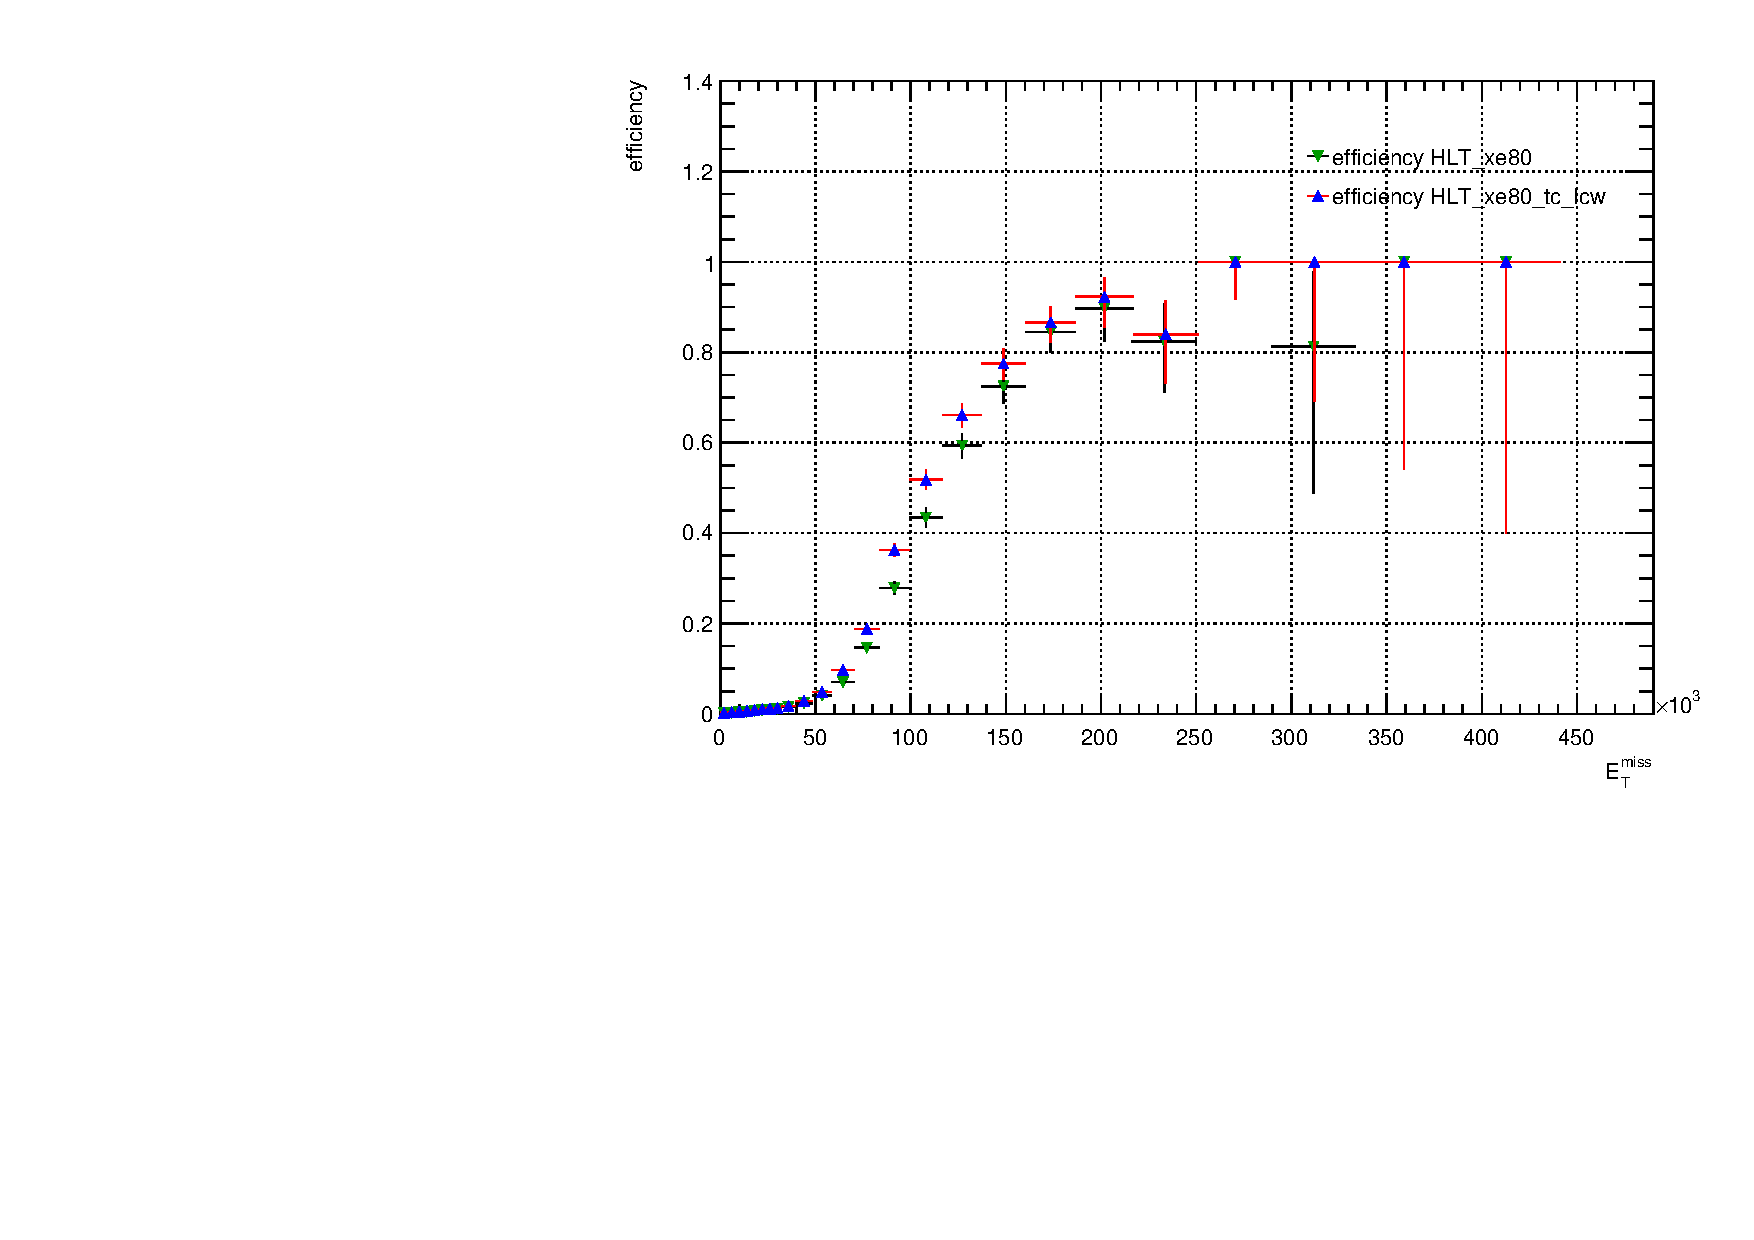
\includegraphics[width=0.49\textwidth]{TRIGGER/Eff_HLT_xe80_HLT_xe80_tc_lcw.pdf}
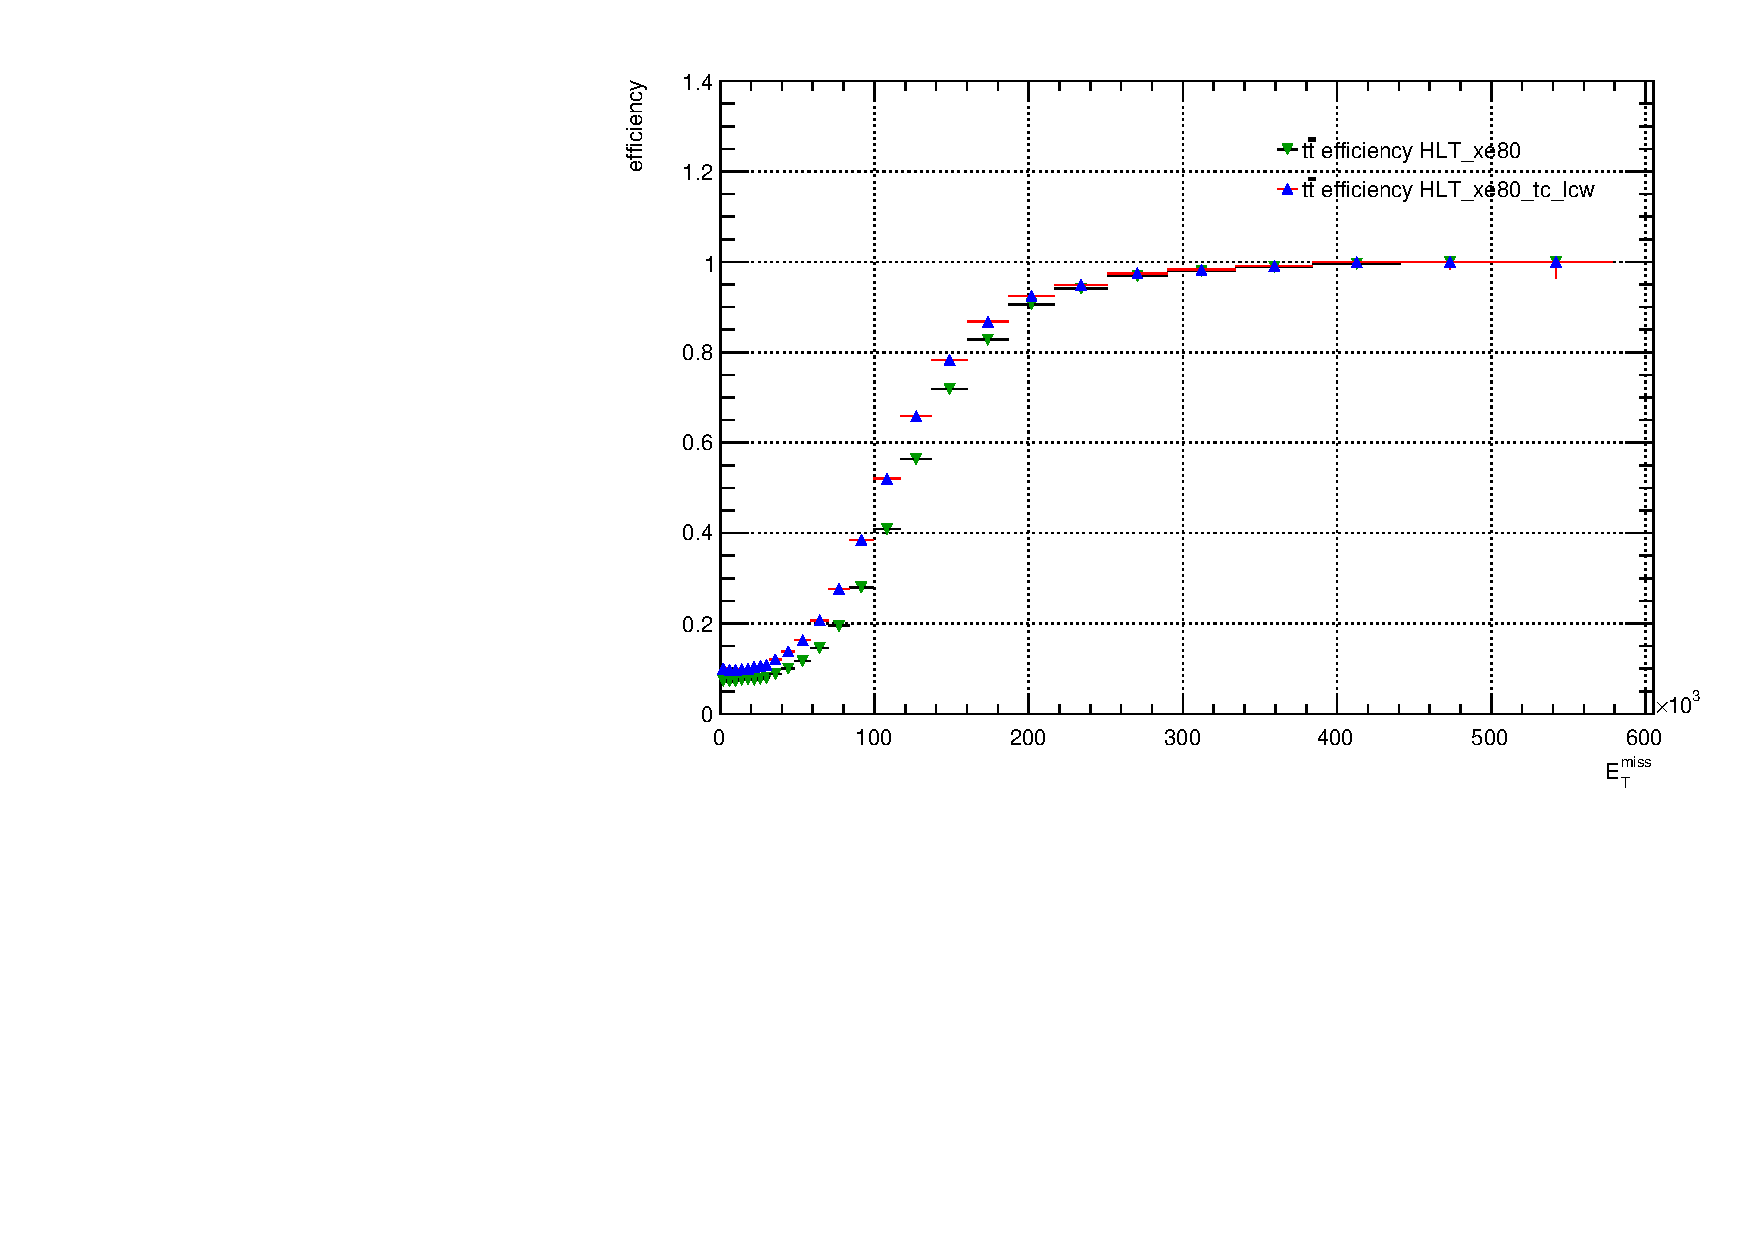
\includegraphics[width=0.49\textwidth]{TRIGGER/Eff_HLT_xe80_HLT_xe80_tc_lcw_MC.pdf}
\caption{Trigger efficiencies for \texttt{HLT\_xe80} and \texttt{HLT\_xe80\_tc\_lcw} versus the missing energy. Shown for the real data events (left) and $t\bar{t}$ Monte Carlo (right)}
\label{fig:triggerEff_HLT_xe80}
\end{figure}

\begin{figure}[htb!]
\centering
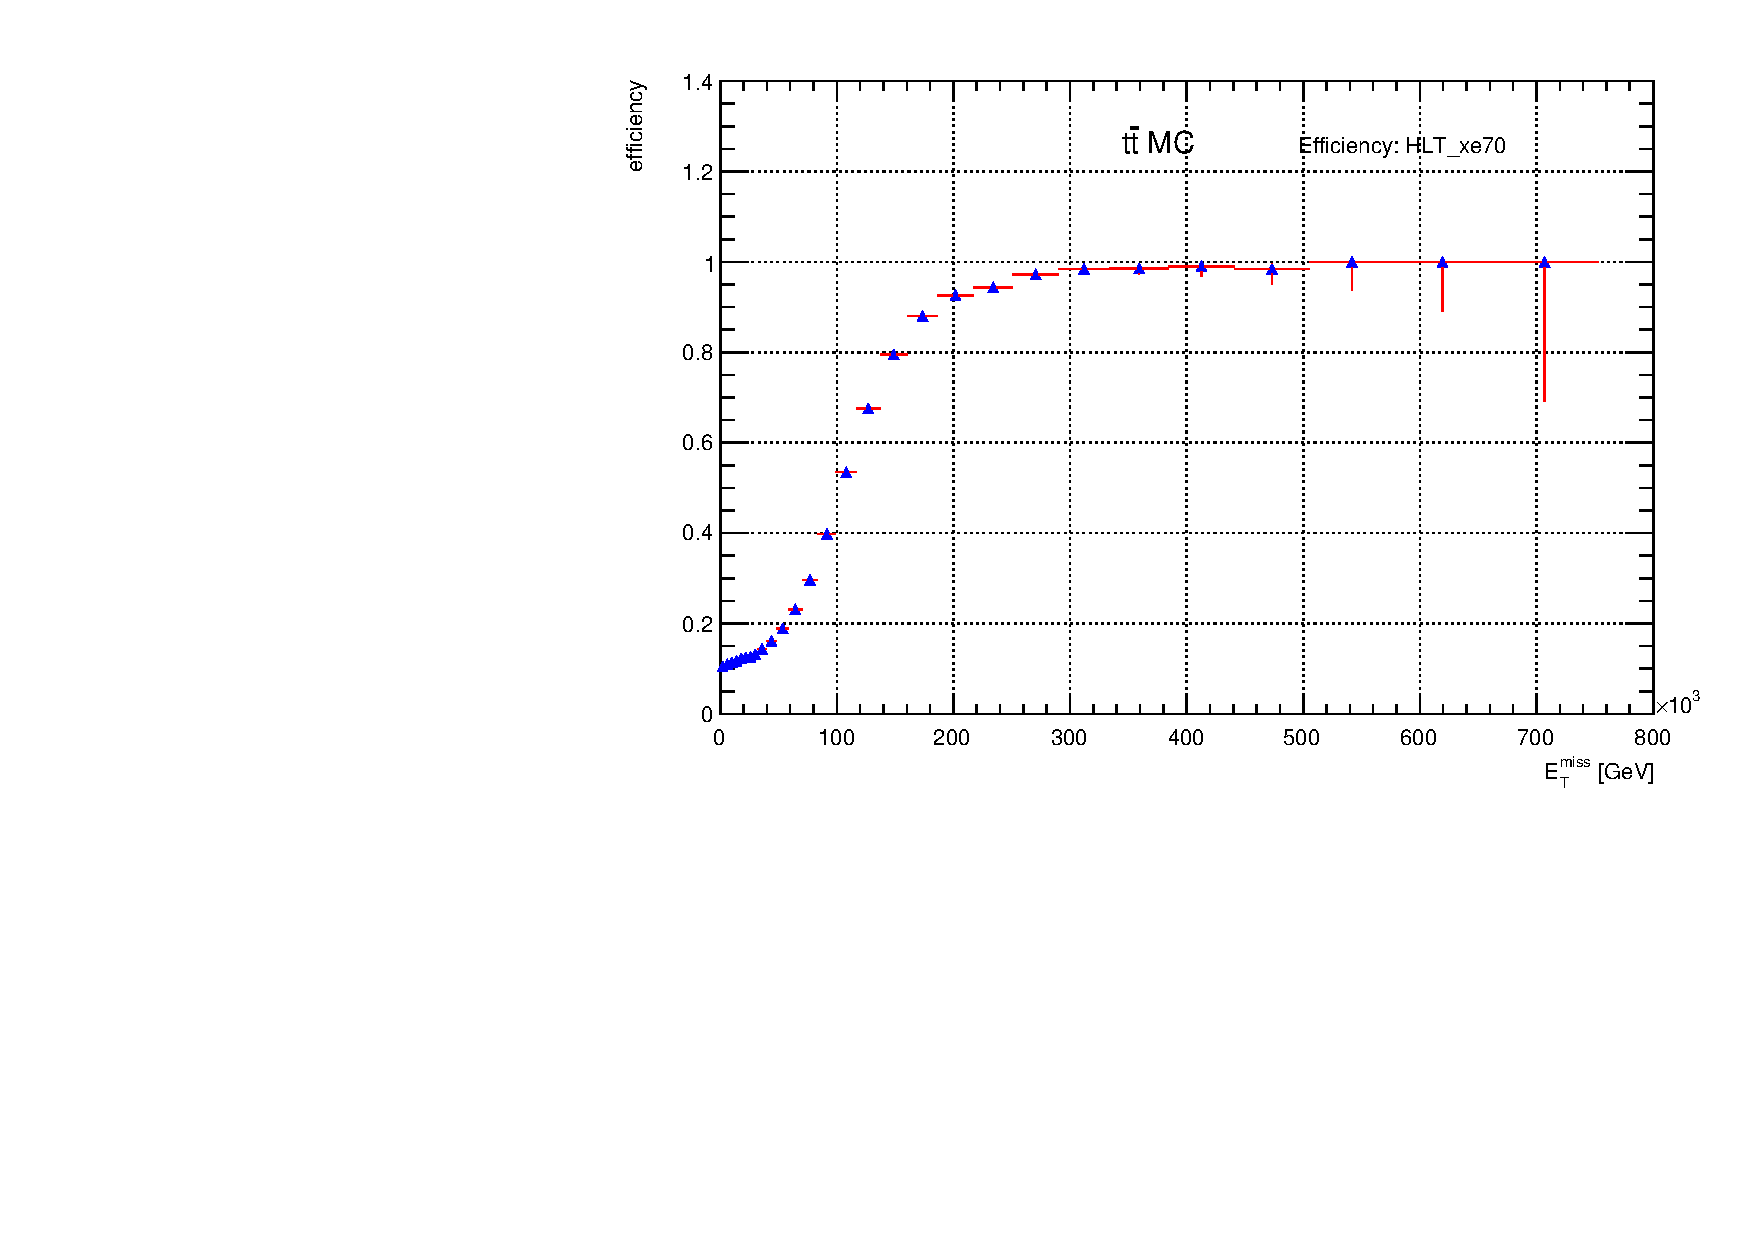
\includegraphics[width=0.49\textwidth]{TRIGGER/Eff_HLT_xe70_MC.pdf}
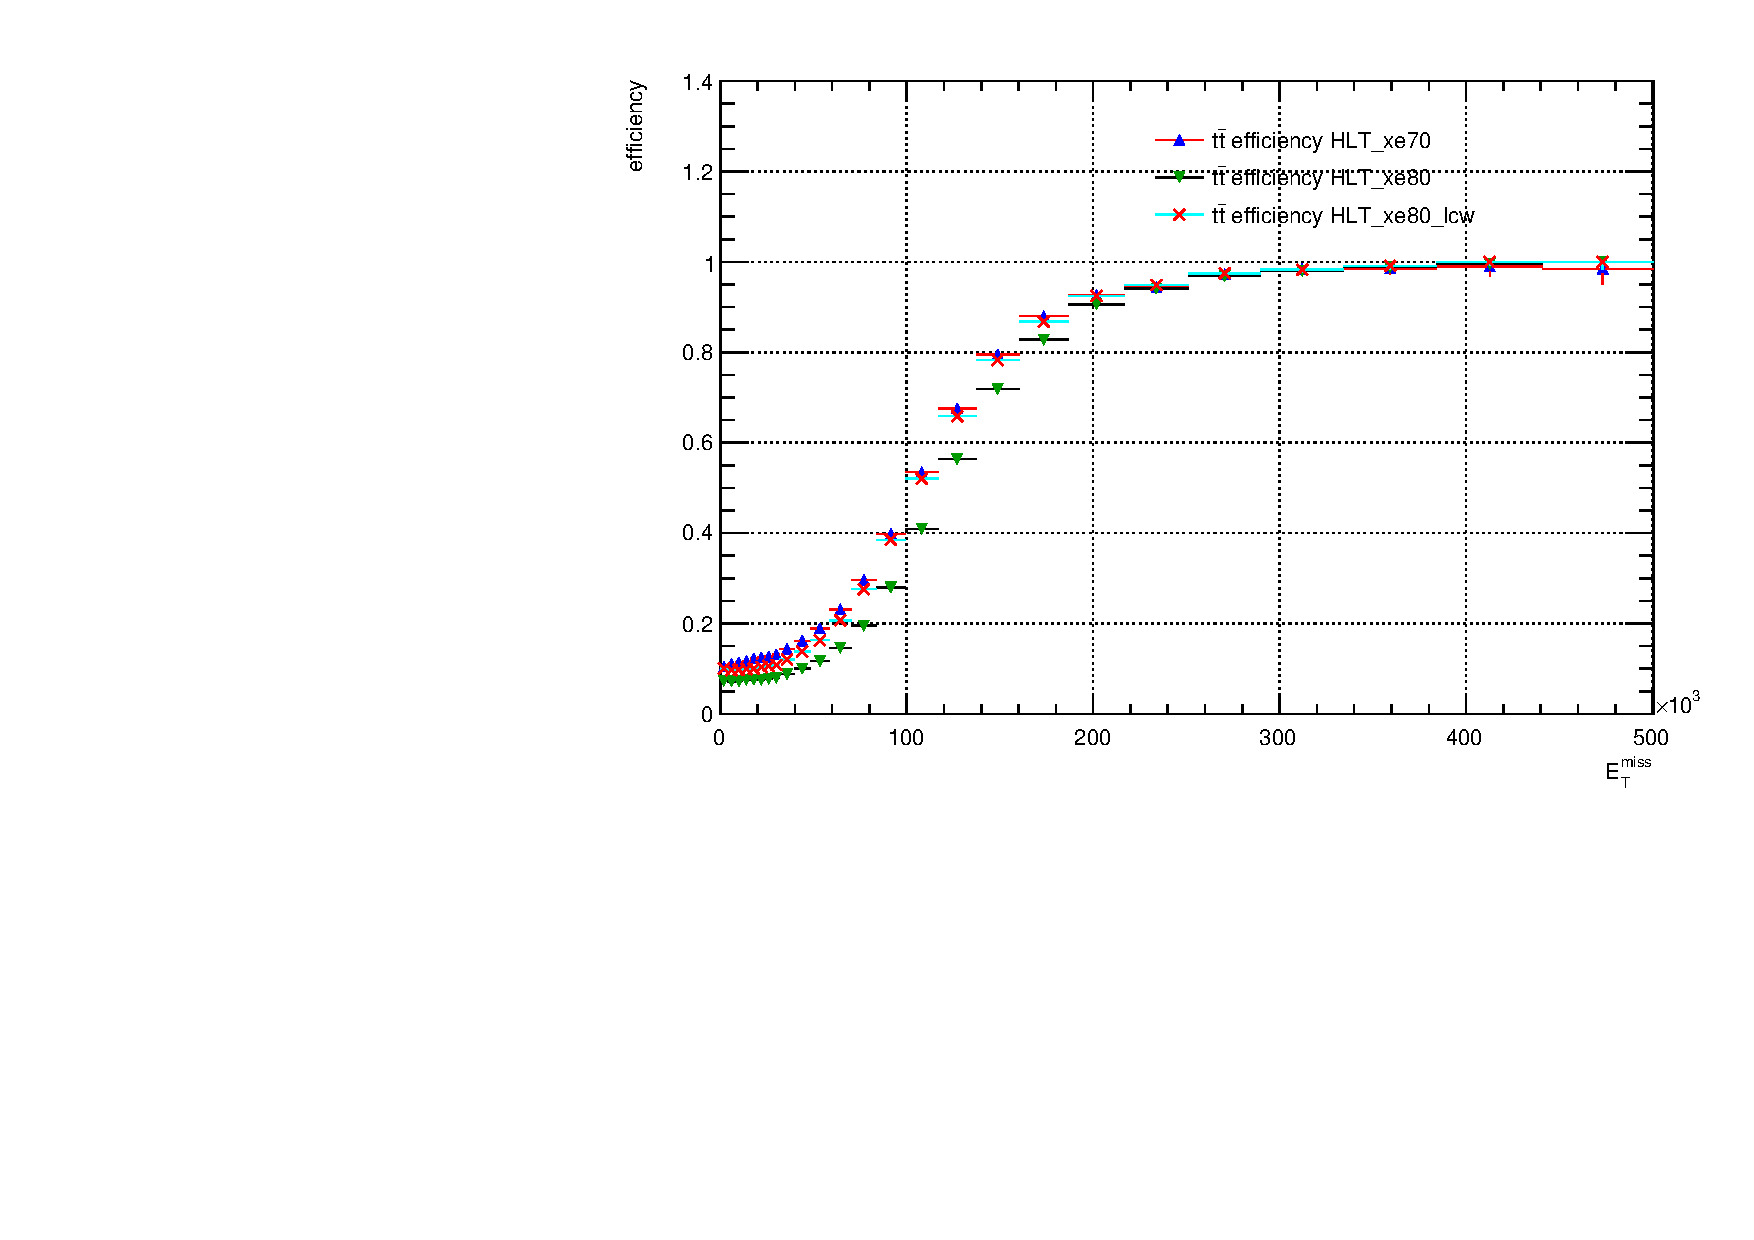
\includegraphics[width=0.49\textwidth]{TRIGGER/Eff_HLT_xe70_HLT_xe80.pdf}
\caption{Trigger efficiencies for \texttt{HLT\_xe70}  versus the missing energy (left). A direct comparision of the efficiency evolution for \texttt{HLT\_xe70} , \texttt{HLT\_xe80} and \texttt{HLT\_xe80\_tc\_lcw} is shown on the right-hand side.  }
\label{fig:triggerEff_HLT_xe70}
\end{figure}


\subsubsection{Dependency on jet requirements}

The several jet requirements in the signal regions of this analysis make it essential to test the trigger efficiency also in events containing additional high $\pt$ jets. The turn-on curves for the  \texttt{HLT\_xe80} and \texttt{HLT\_xe80\_tc\_lcw} trigger by asking for one, two or three jets with $\pt > 50$ GeV in addition to the missing $E_T$ are shown in figure~\ref{fig:triggerEff_HLT_xe80_jets}. The same plot for \texttt{HLT\_xe70} is shown on figure~\ref{fig:triggerEff_HLT_xe70_jets}. This study is only shown for $t\bar{t}$ Monte Carlo, since the selection of these events leads to lower numbers of selected events and therefore to higher statistical uncertainties in the investigated dataset. A small dependency of the efficiency evolution can be observed for the additional jet selection criteria. However, if the missing $E_T$ is above 250 GeV, the effect is smaller than $5\%$.


\begin{figure}[htb!]
\centering
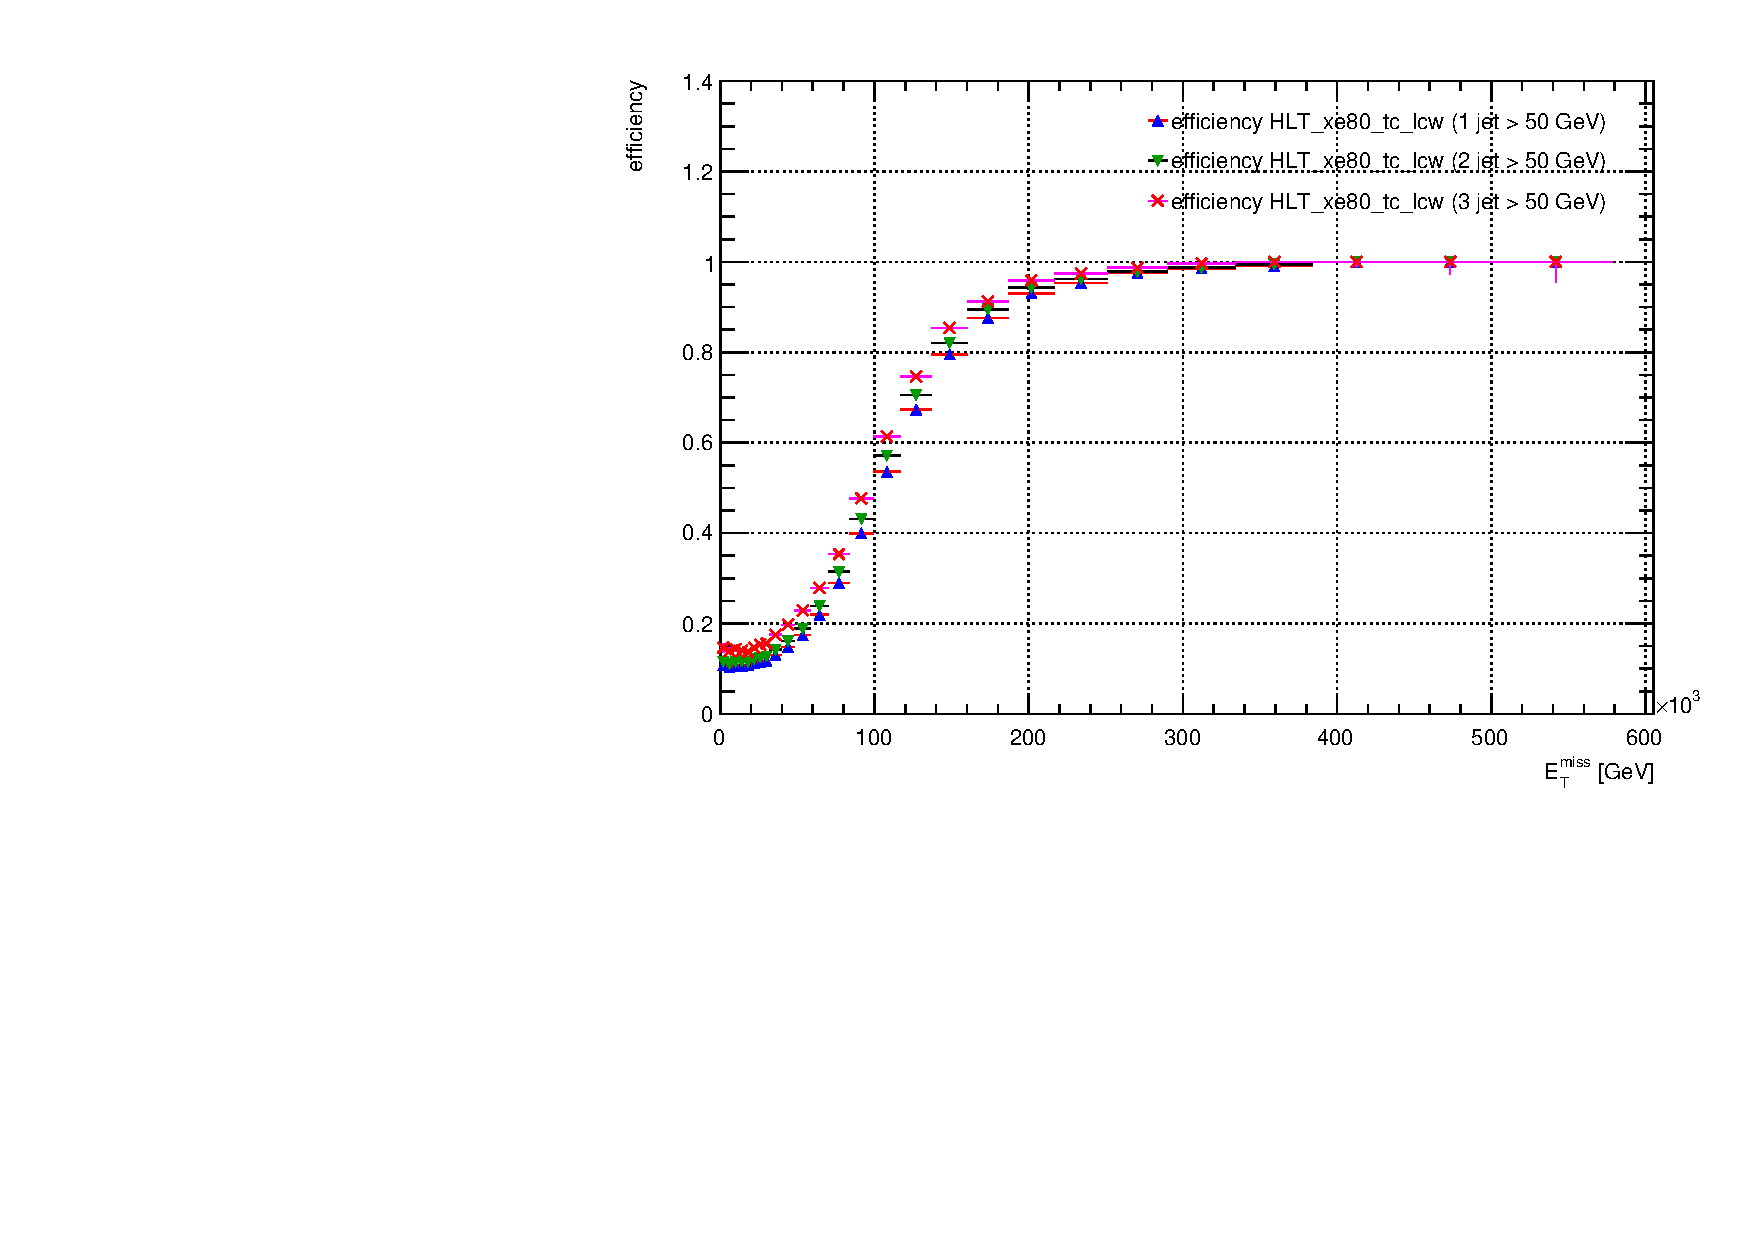
\includegraphics[width=0.49\textwidth]{TRIGGER/Eff_HLT_xe80_tc_lcw_jets_MC.pdf}
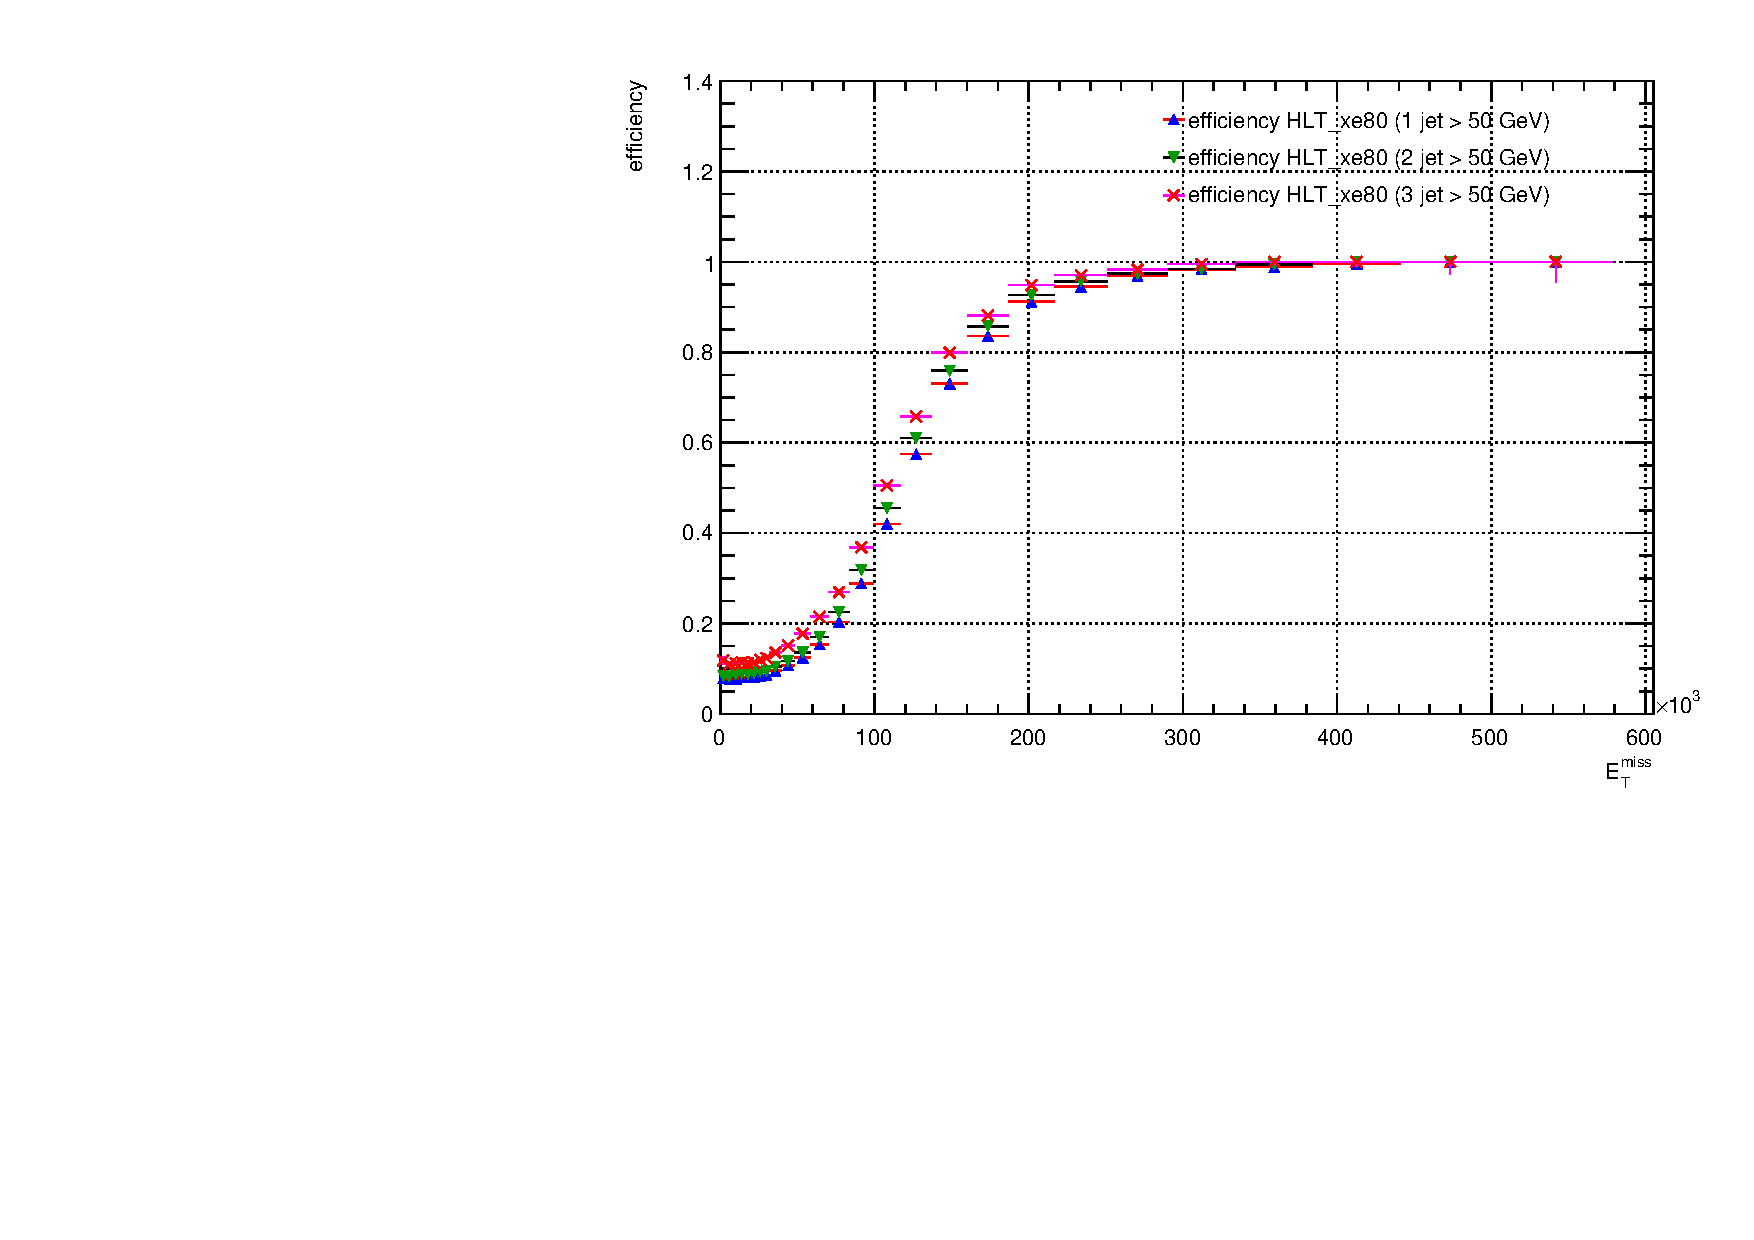
\includegraphics[width=0.49\textwidth]{TRIGGER/Eff_HLT_xe80_jets_MC.pdf}
\caption{Trigger efficiencies for \texttt{HLT\_xe80\_tc\_lcw} (left) and \texttt{HLT\_xe80} (right) versus the missing energy by requiring one, two or three additional jets with $\pt > 50$ GeV. Also in this case a preselection of events containing two leptons with $\pt > 10 $ GeV is applied.}
\label{fig:triggerEff_HLT_xe80_jets}
\end{figure}

\begin{figure}[htb!]
\centering
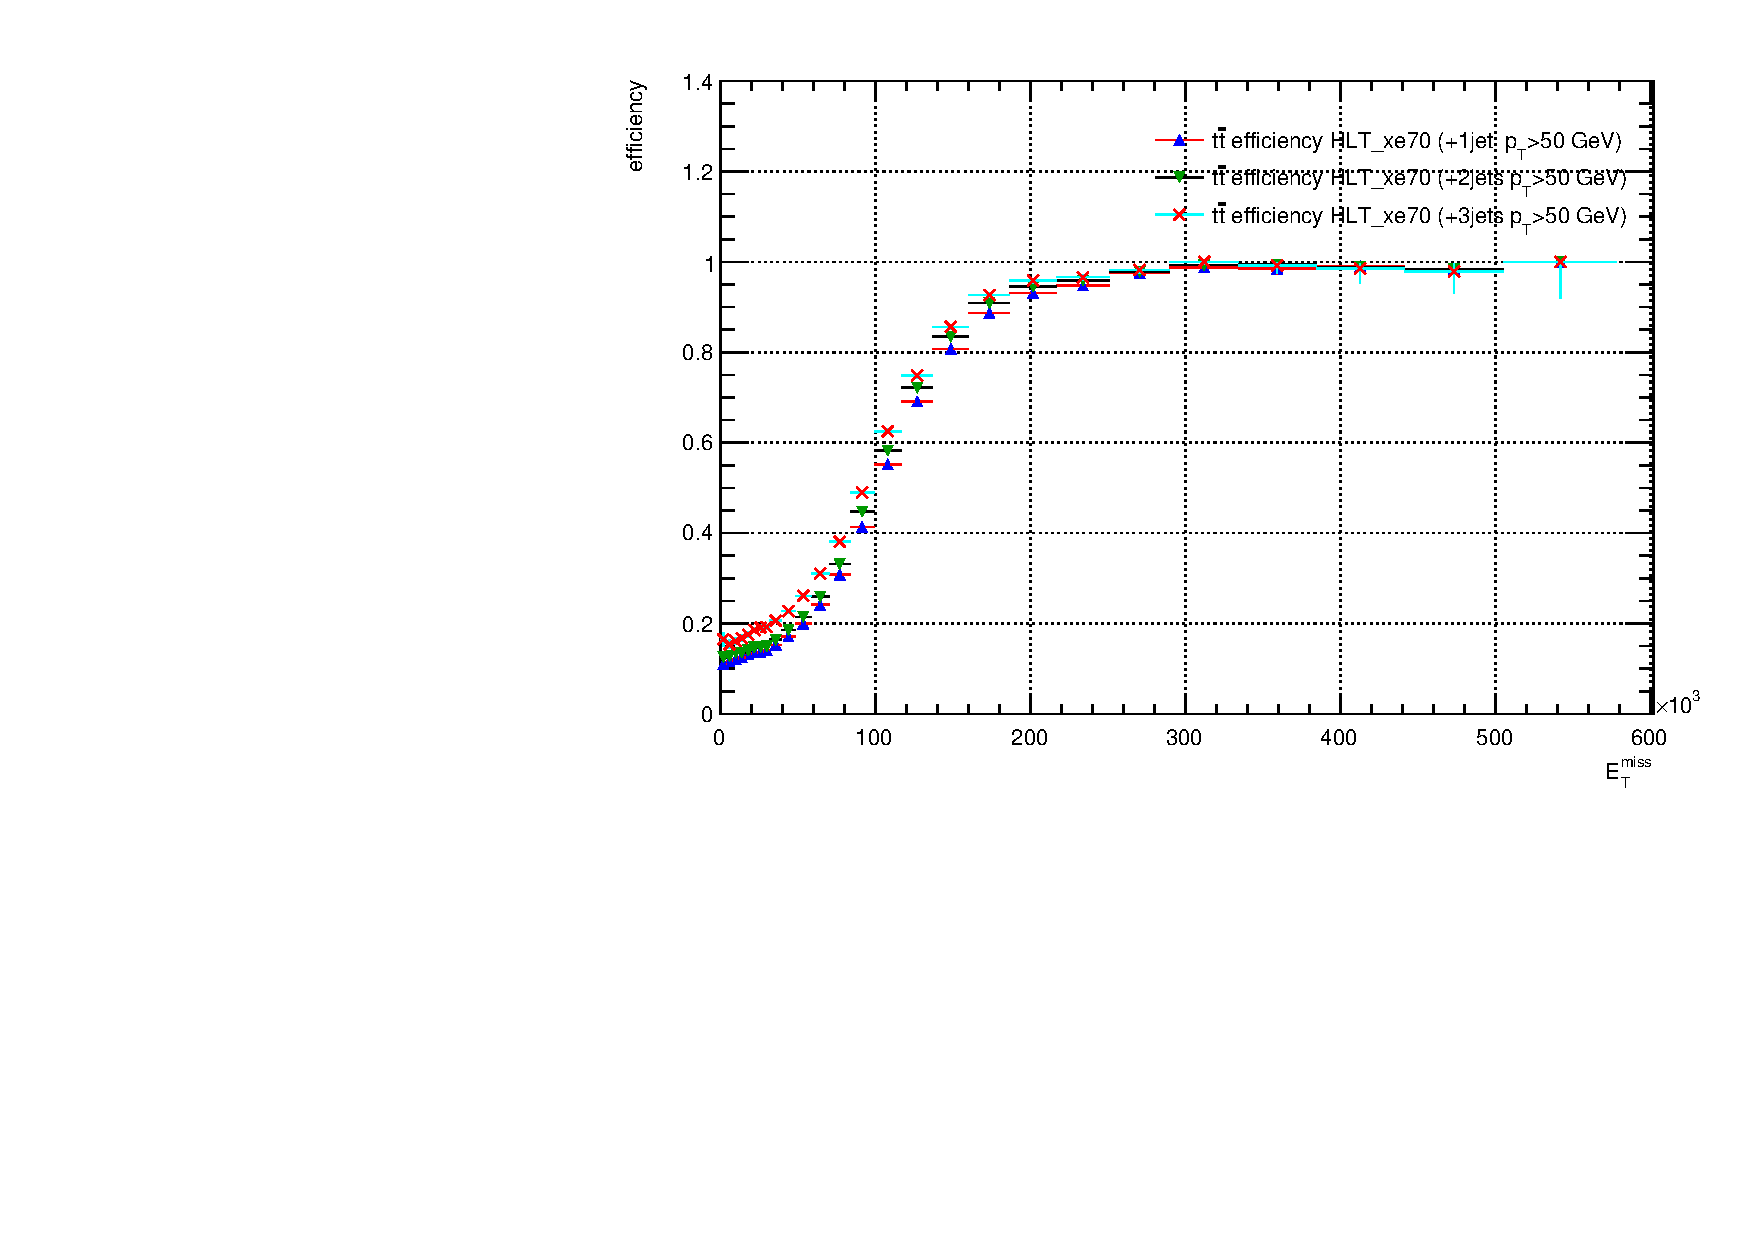
\includegraphics[width=0.50\textwidth]{TRIGGER/Eff_HLT_xe70_jets_MC.pdf}
\caption{Trigger efficiency for \texttt{HLT\_xe70} versus the missing energy by requiring one, two or three additional jets with $\pt > 50$ GeV.}
\label{fig:triggerEff_HLT_xe70_jets}
\end{figure}


\subsubsection{Inefficiency issues of $\met$ triggers}

Both triggers show small inefficiencies for high $\met$ values. A probable reason for this is that muons are not included in the L1 $\met$ value used for the online trigger decision. To understand this effect, the requirement of the lepton pair with $\pt > 10 $ GeV has been separated by the lepton flavor. This provides a separate measurement of efficiencies for events containing electrons and muons. The efficiencies are shown in figure~\ref{fig:triggerEff_leptons_MC} for $t\bar{t}$ Monte Carlo and figure~\ref{fig:triggerEff_leptons_DATA} for data events.

It is obvious that the measurements using di-muon events show some inefficiencies with respect to the di-electron events. This supports the presumption that the missing muons at the L1 trigger $\met$ are responsible for the inefficiencies observed in all $\met$ triggers investigated. However, since we will combine the $\met$- and the di-lepton triggers with a logical \texttt{OR} for the event selection in the analysis, these events should be selected by the di-lepton triggers. Additional plots are shown in~\ref{app_HLT_xe80}.

\begin{figure}[htb!]
\centering
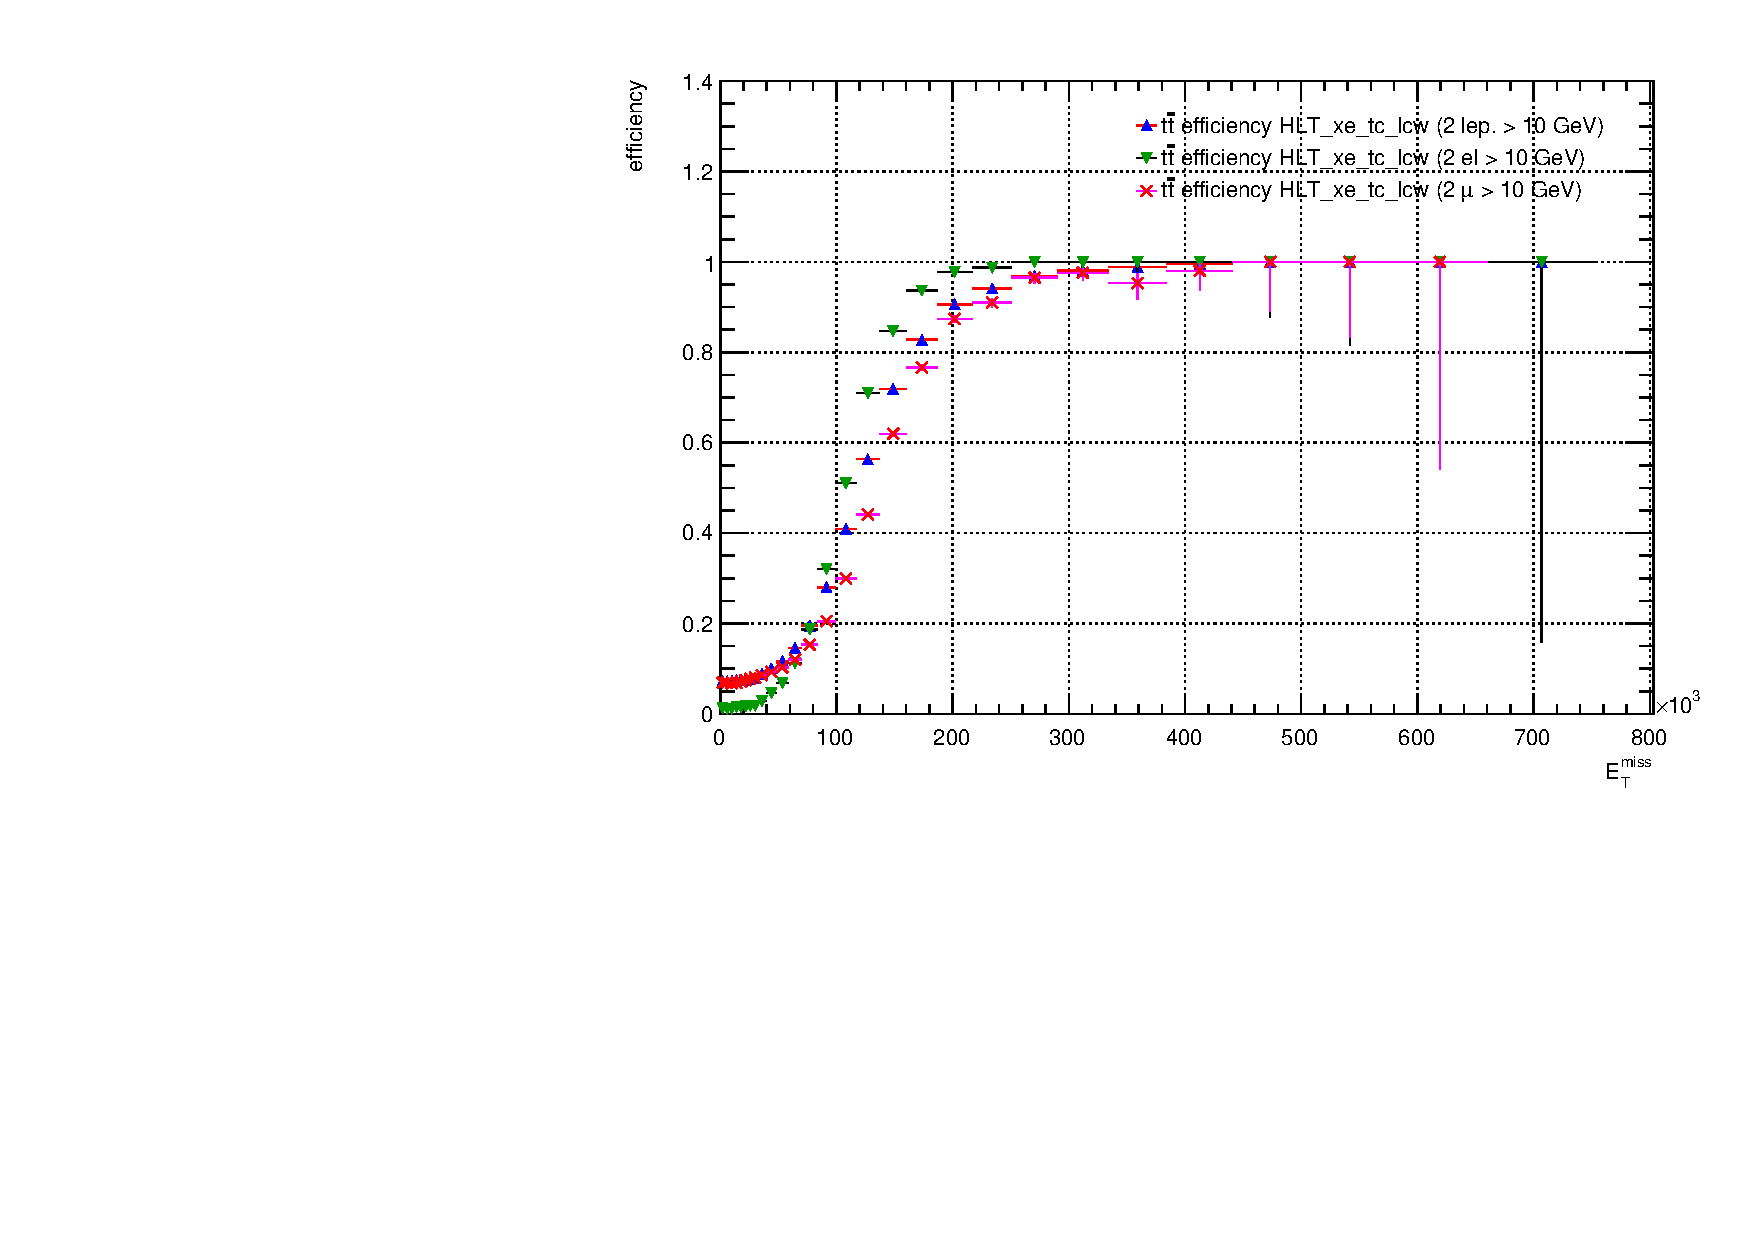
\includegraphics[width=0.49\textwidth]{TRIGGER/Eff_HLTxe80_tc_lcw_ElMu.pdf}
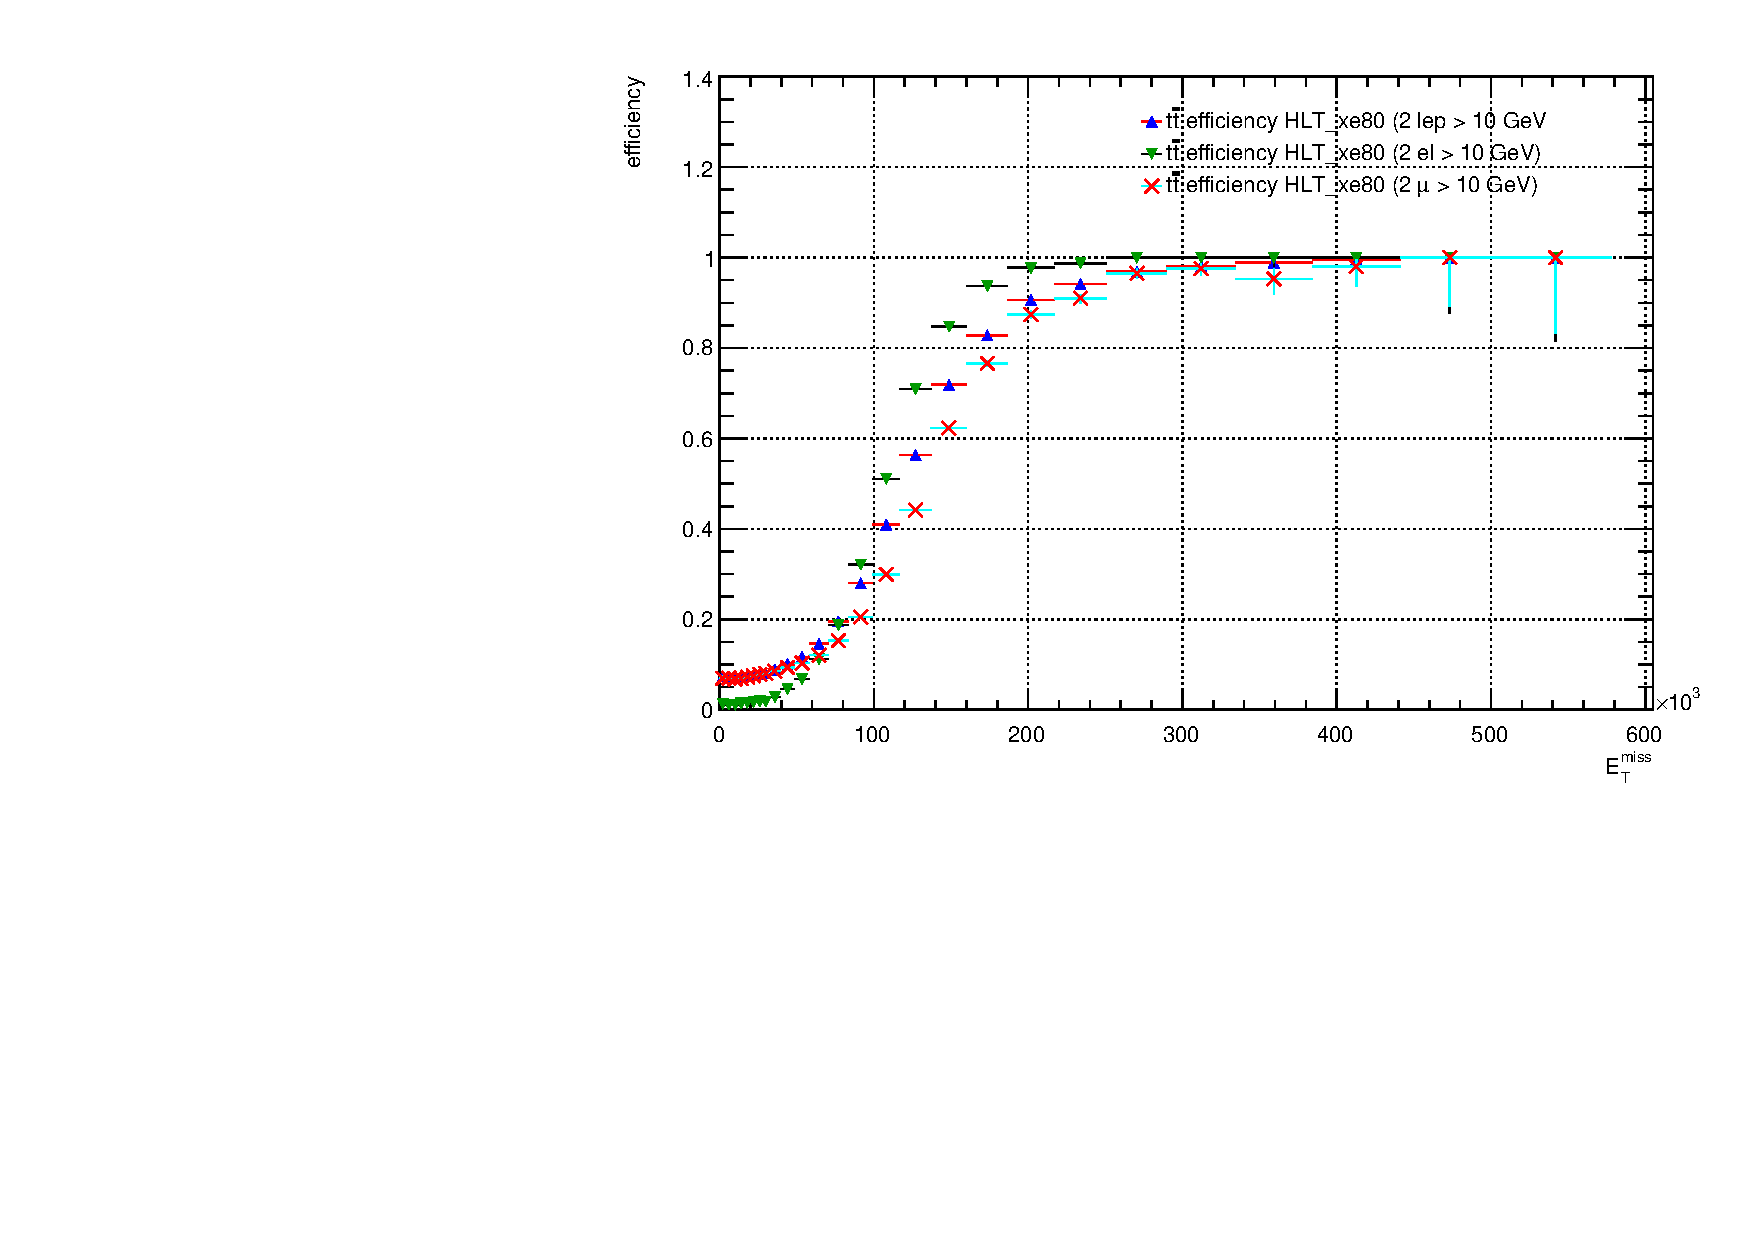
\includegraphics[width=0.49\textwidth]{TRIGGER/Eff_HLTxe80_ElMu.pdf}
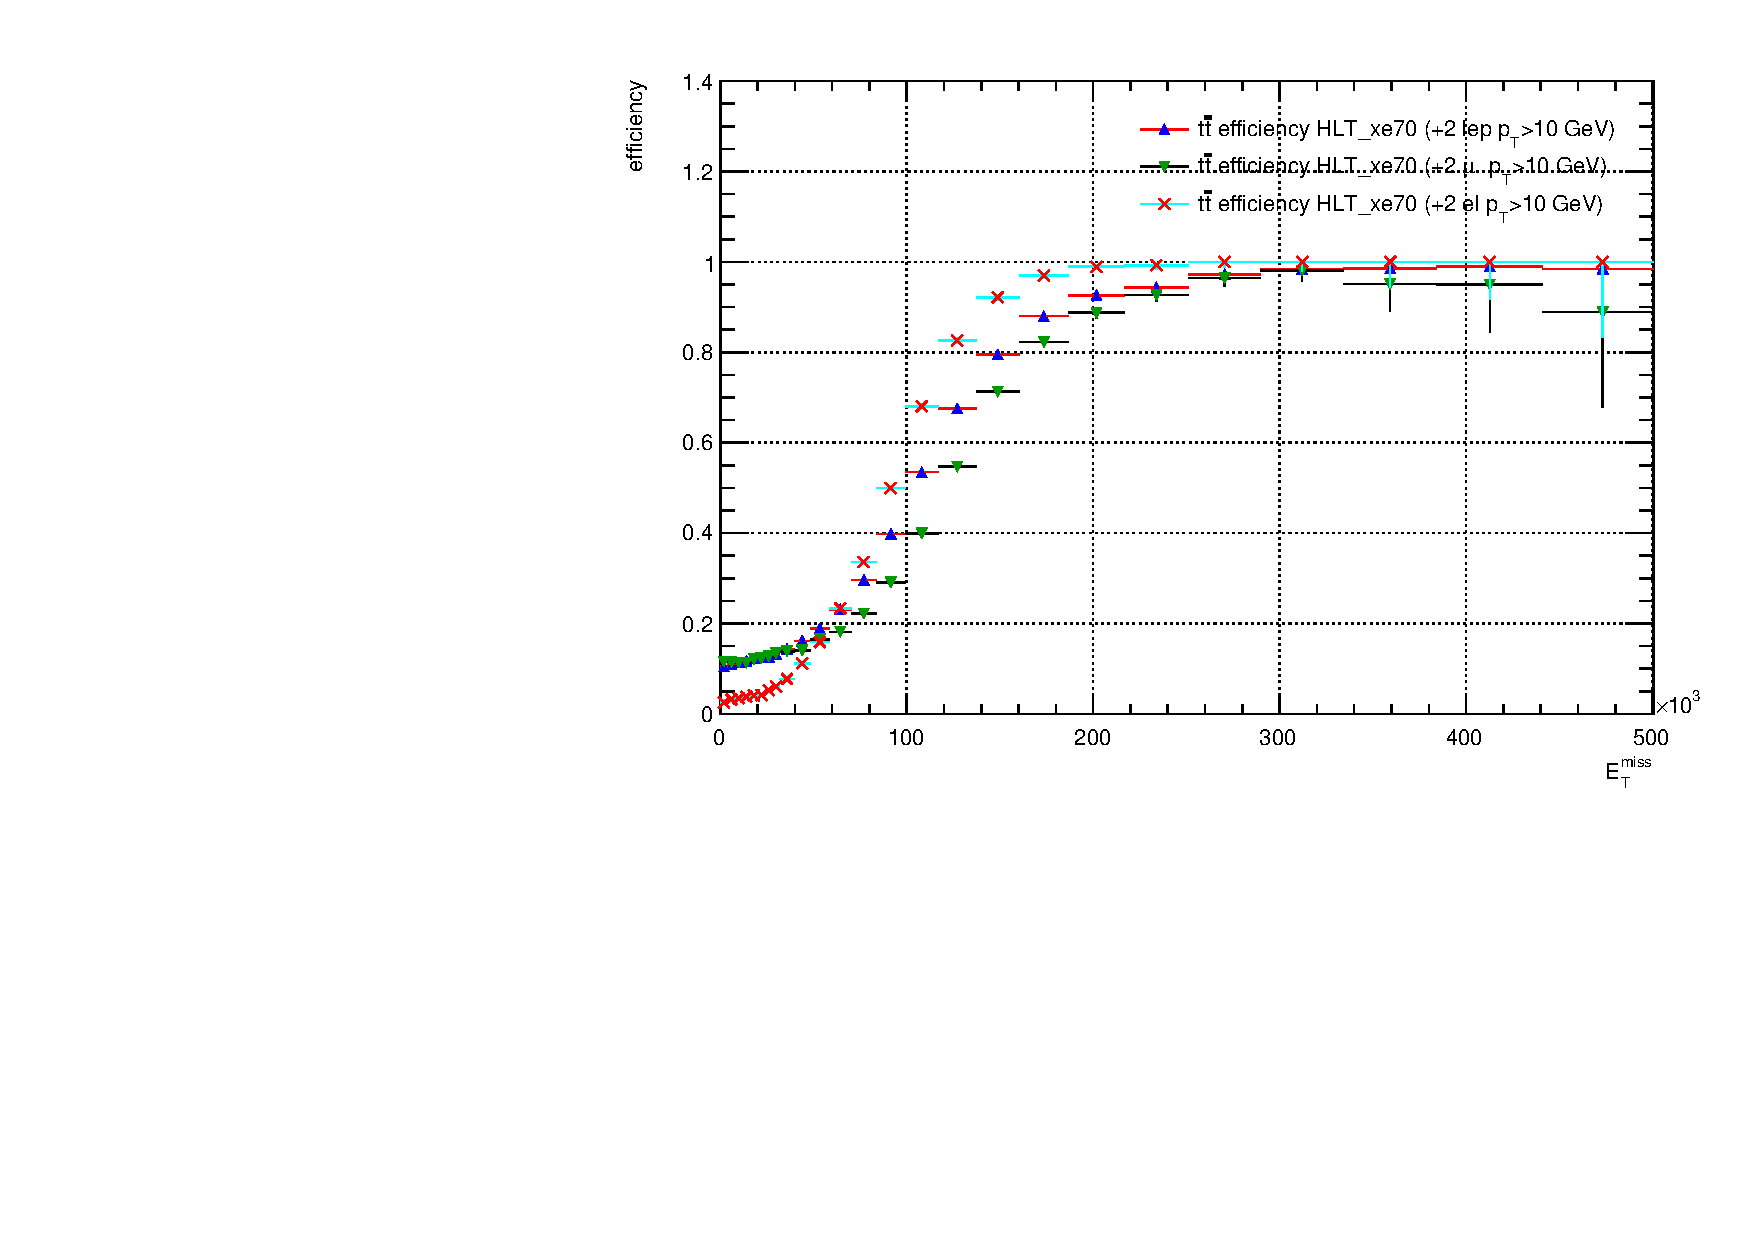
\includegraphics[width=0.49\textwidth]{TRIGGER/Eff_HLT_xe70_ElMu_MC.pdf}
\caption{Trigger efficiencies for \texttt{HLT\_xe80\_tc\_lcw} (top-left),  \texttt{HLT\_xe80} (top-right) and \texttt{HLT\_xe80} (bottom) versus $\met$ obtained from $t\bar{t}$ Monte Carlo. The different curves show the efficiency for events containing a $ll$, $ee$ or $\mu\mu$ pair.}
\label{fig:triggerEff_leptons_MC}
\end{figure}

\begin{figure}[htb!]
\centering
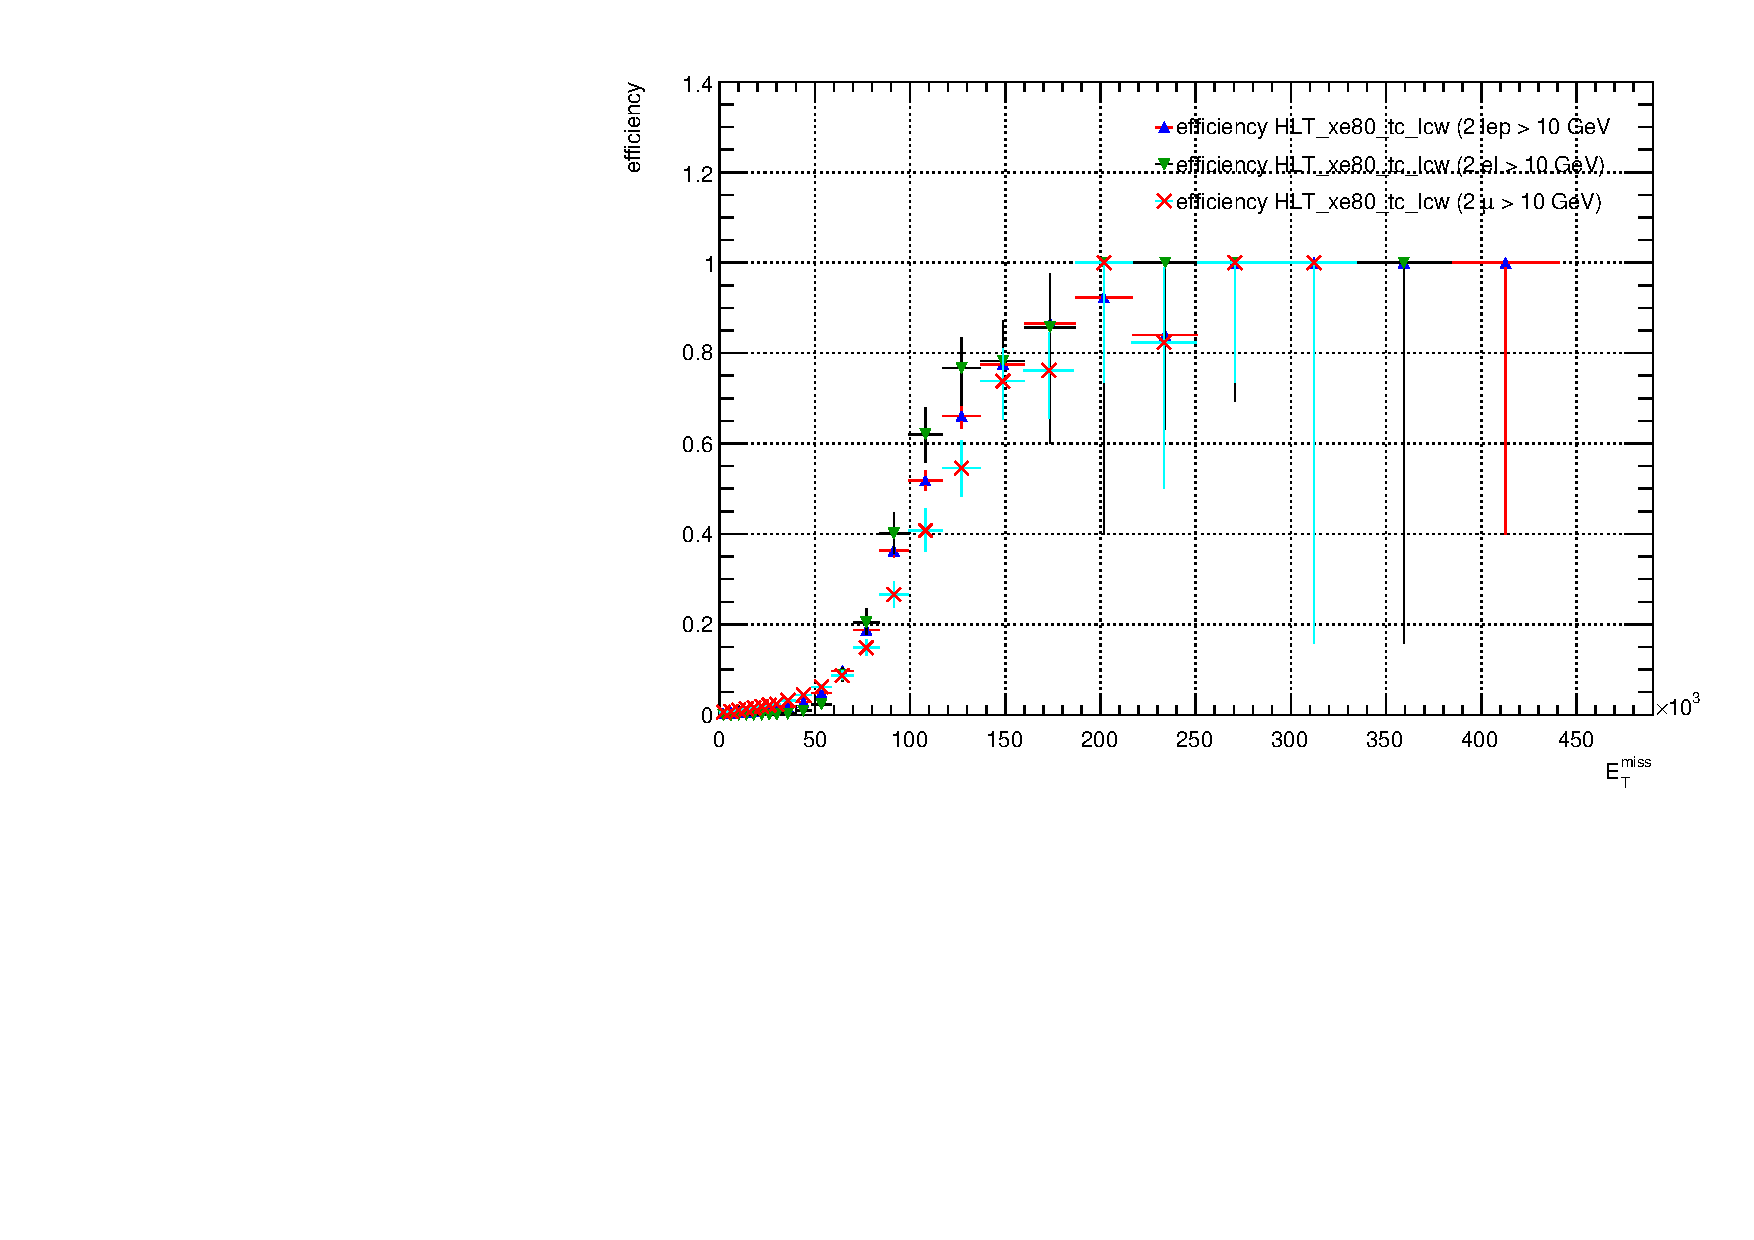
\includegraphics[width=0.49\textwidth]{TRIGGER/Eff_HLTxe80_tc_lcw_Data_ElMu.pdf}
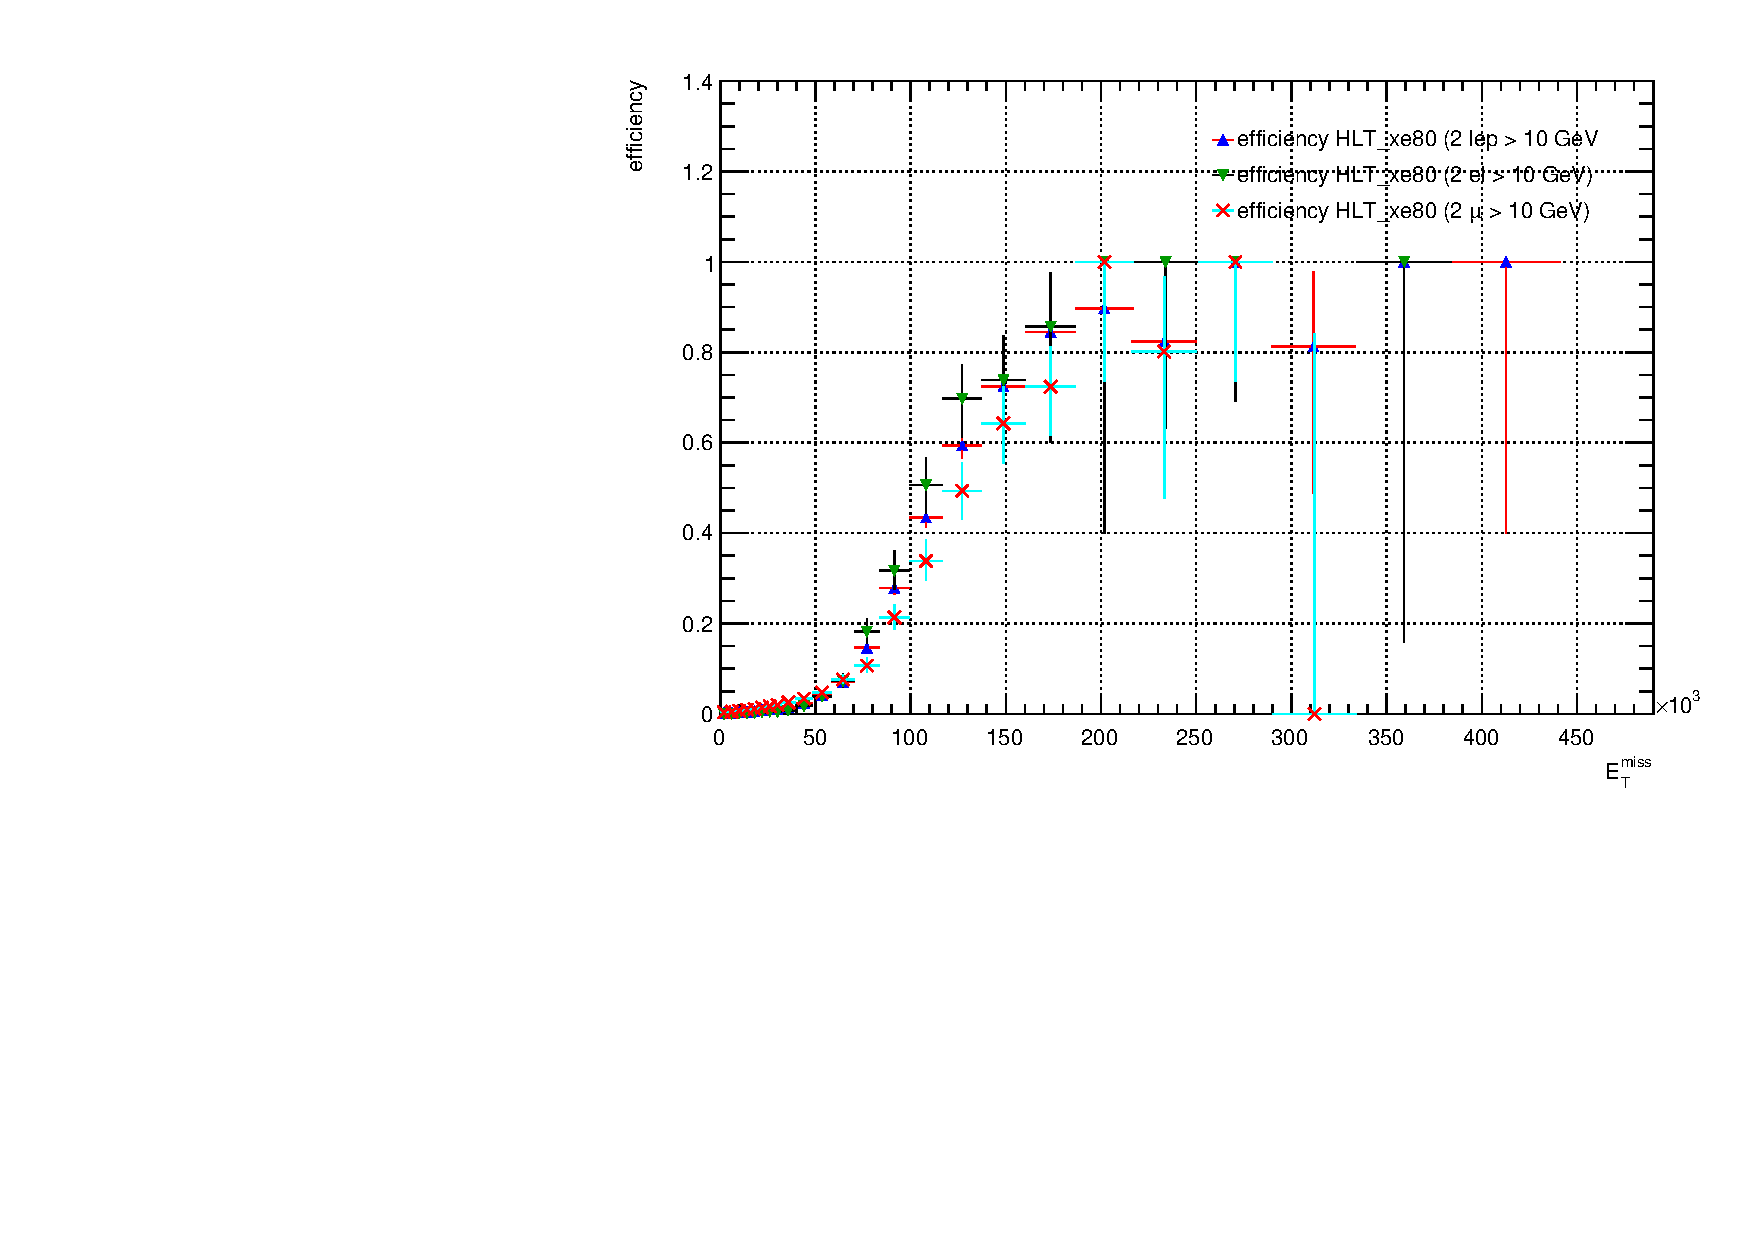
\includegraphics[width=0.49\textwidth]{TRIGGER/Eff_HLTxe80_Data_ElMu.pdf}
\caption{Trigger efficiencies in data for \texttt{HLT\_xe80\_tc\_lcw} (left) and \texttt{HLT\_xe80} (right) versus $\met$. The different curves show the efficiency for events containing a $ll$, $ee$ or $\mu\mu$ pair.}
 \label{fig:triggerEff_leptons_DATA}
\end{figure}

Based on these studies and efficiency measurements, a preliminary decision for the trigger selection has been made.

\begin{itemize}

\item If $\met$ < 250 GeV, only and \texttt{OR} combination of di-lepton triggers is used. 

\item If $\met$ > 250 GeV, an \texttt{OR} between the di-lepton triggers and \texttt{HLT\_xe70} is used.

\end{itemize}



\clearpage
\section{Selected events and efficicency plot for $\met$ trigger}
\label{app_HLT_xe80}

Studies on performance and efficiency have been done for \texttt{HLT\_xe80} and \texttt{HLT\_xe80\_tc\_lcw}. Efficiency plots and histograms showing the triggered events can be found here. 

\begin{figure}[h!]
\centering
\subfigure{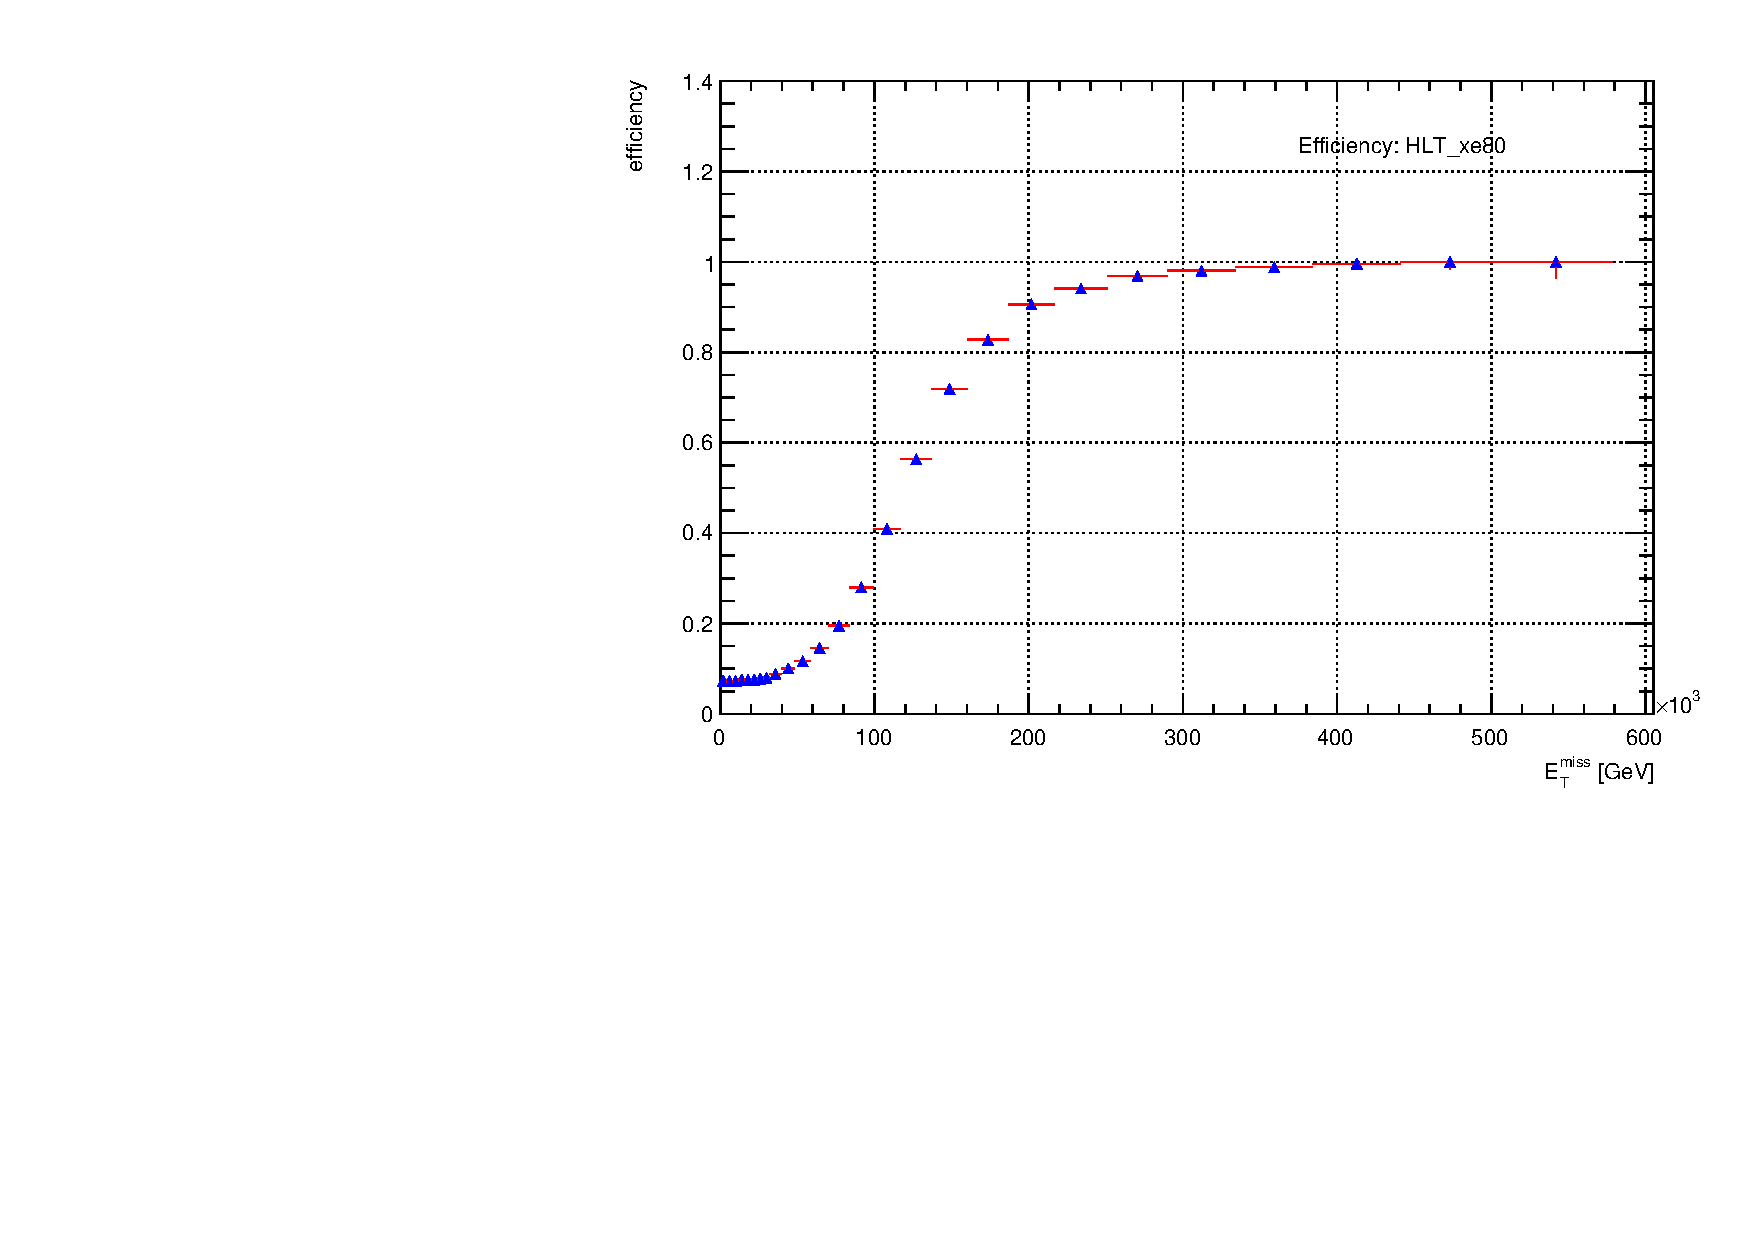
\includegraphics[width=0.42\textwidth]{TRIGGER/Eff_HLT_xe80_MC.pdf}}
\subfigure{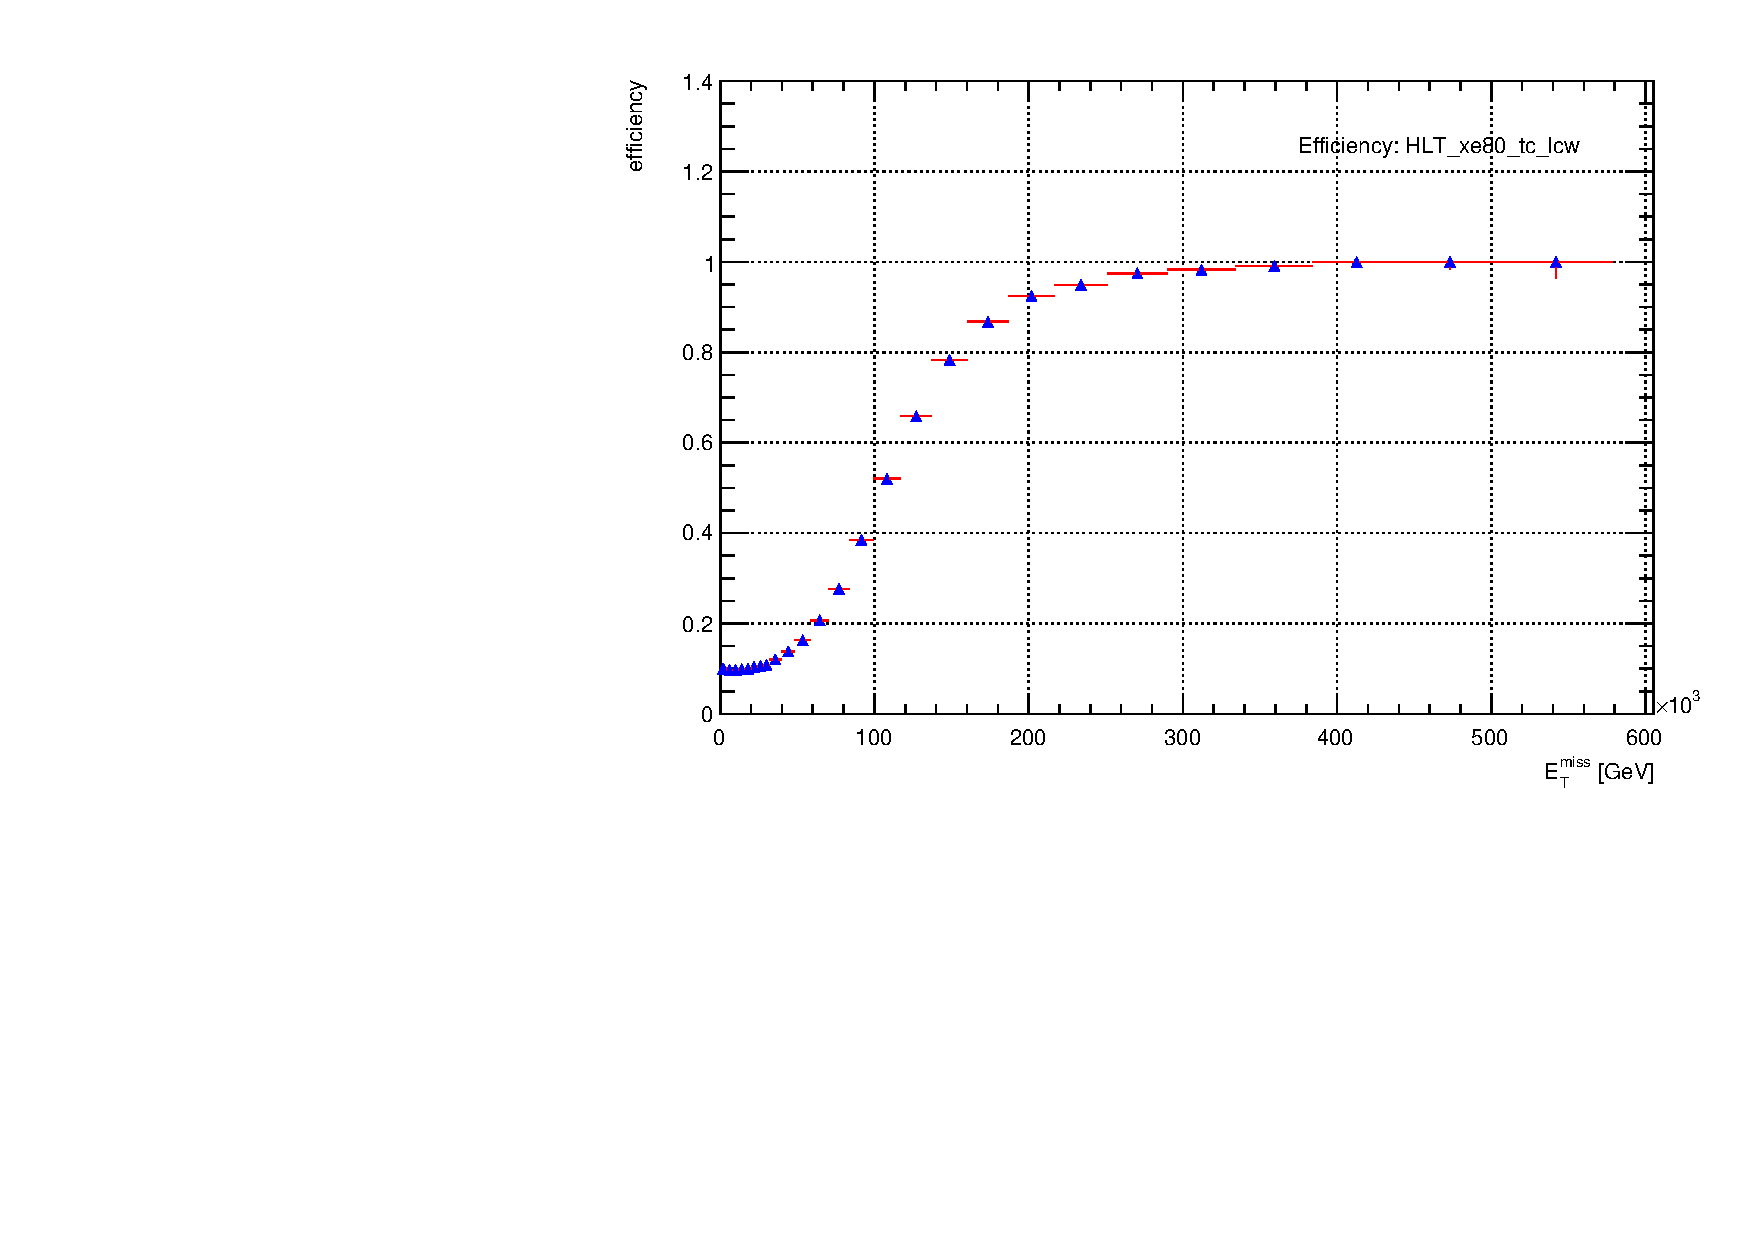
\includegraphics[width=0.42\textwidth]{TRIGGER/Eff_HLT_xe80_tc_lcw_MC.pdf}}
\caption{Efficiency of \texttt{HLT\_xe80} (left) and \texttt{HLT\_xe80\_tc\_lcw} (right) versus the missing energy obtained from $t\bar{t}$ Monte Carlo}
\label{fig:eff_trigger1}
\end{figure}

\begin{figure}[h!]
\centering
\subfigure{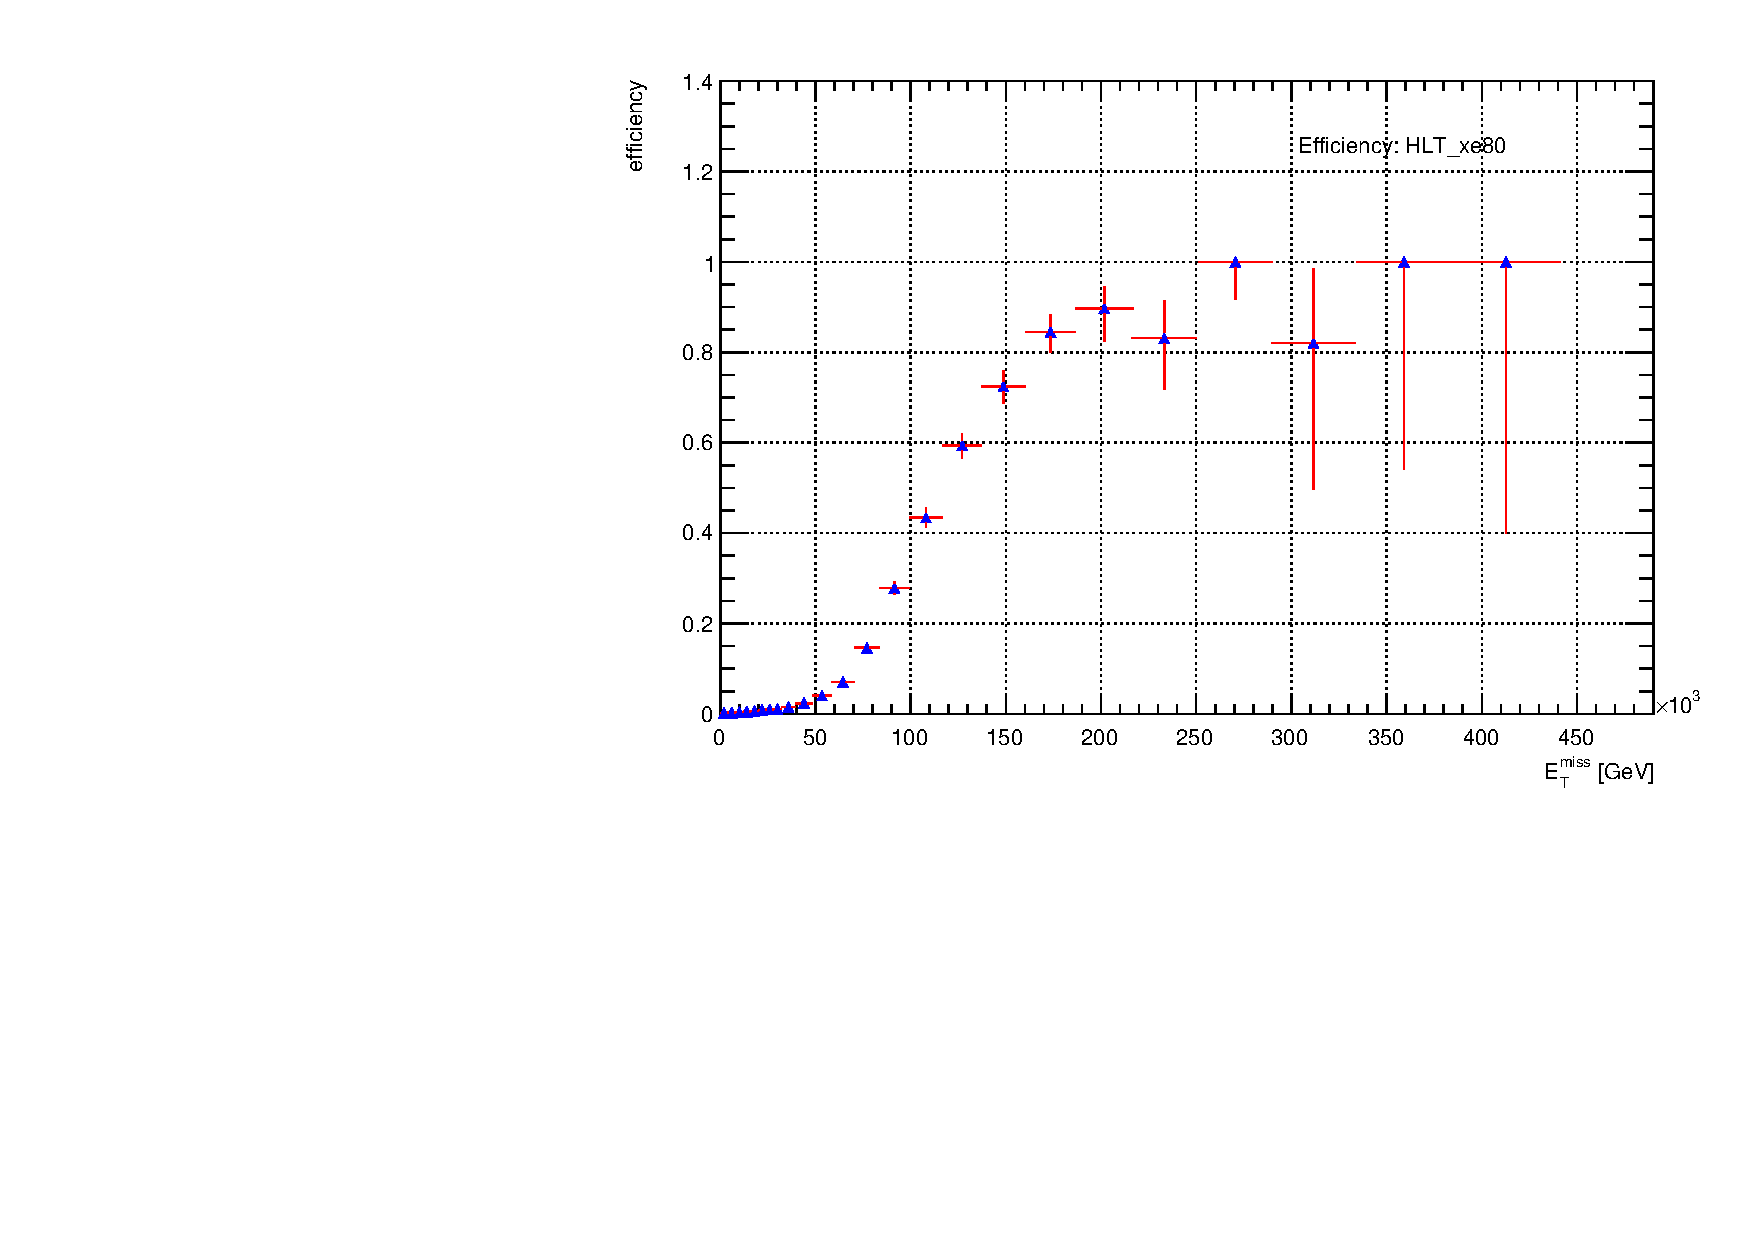
\includegraphics[width=0.42\textwidth]{TRIGGER/Eff_HLT_xe80_Data.pdf}}
\subfigure{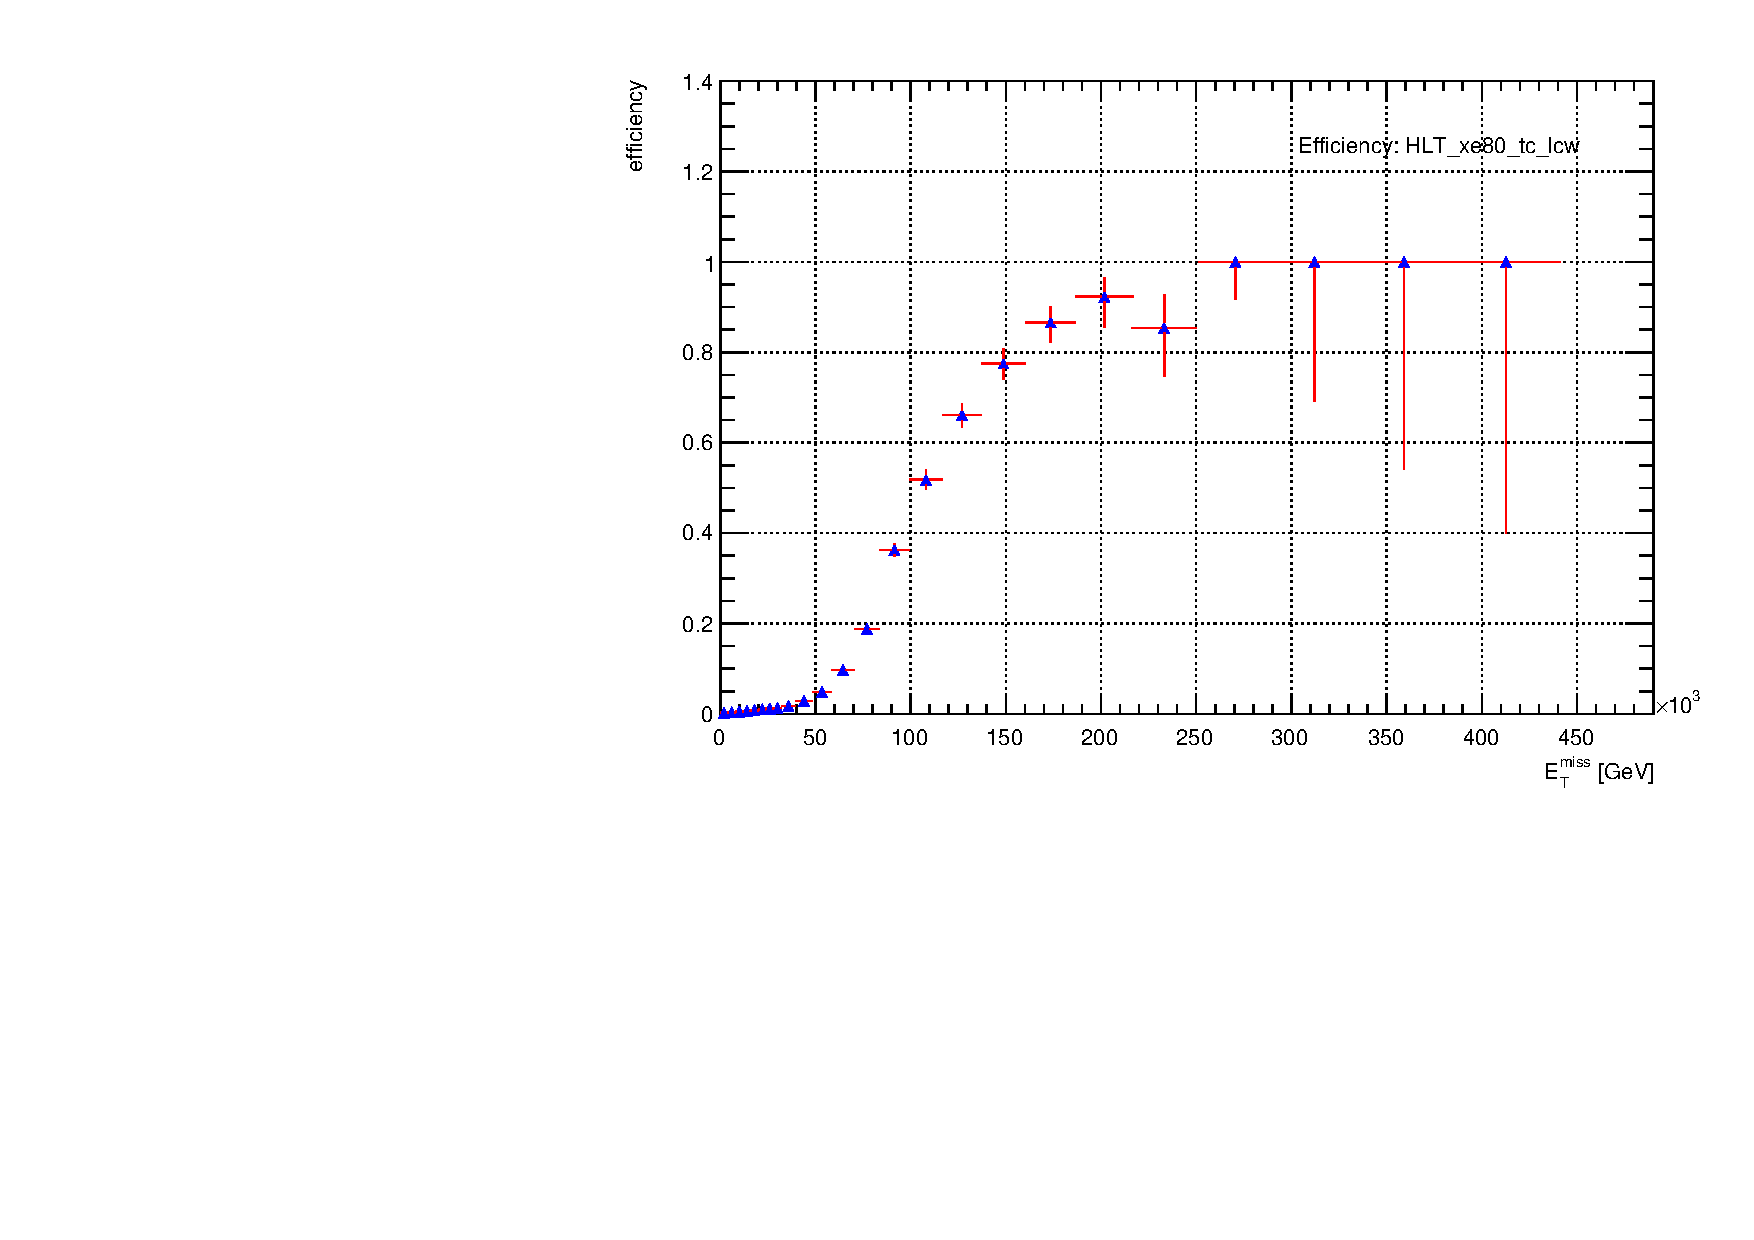
\includegraphics[width=0.42\textwidth]{TRIGGER/Eff_HLT_xe80_tc_lcw_Data.pdf}}
\caption{Efficiency of \texttt{HLT\_xe80} (left) and \texttt{HLT\_xe80\_tc\_lcw} (right) versus the missing energy obtained from data}
\label{fig:eff_trigger2}
\end{figure}

\begin{figure}[h!]
\centering
\subfigure{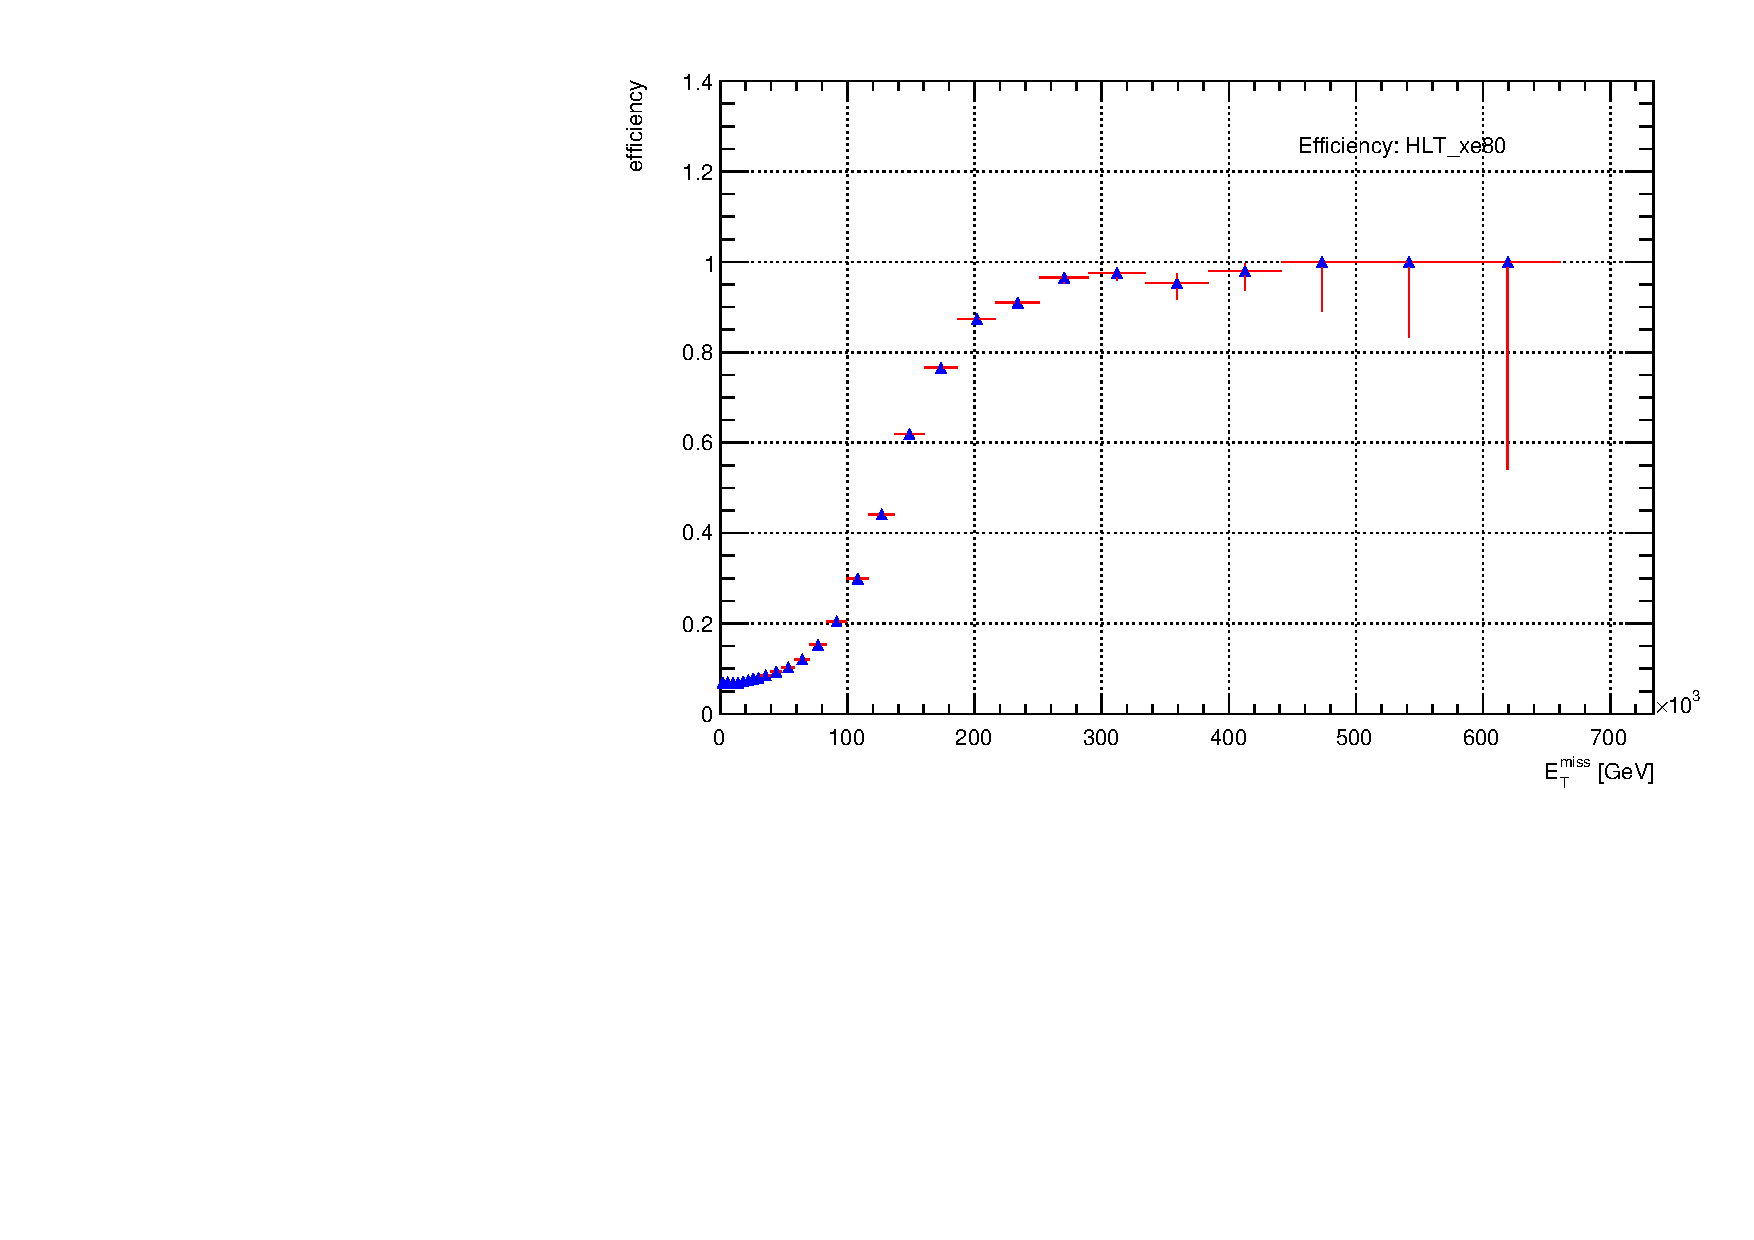
\includegraphics[width=0.42\textwidth]{TRIGGER/Eff_HLT_xe80_Mu_MC.pdf}}
\subfigure{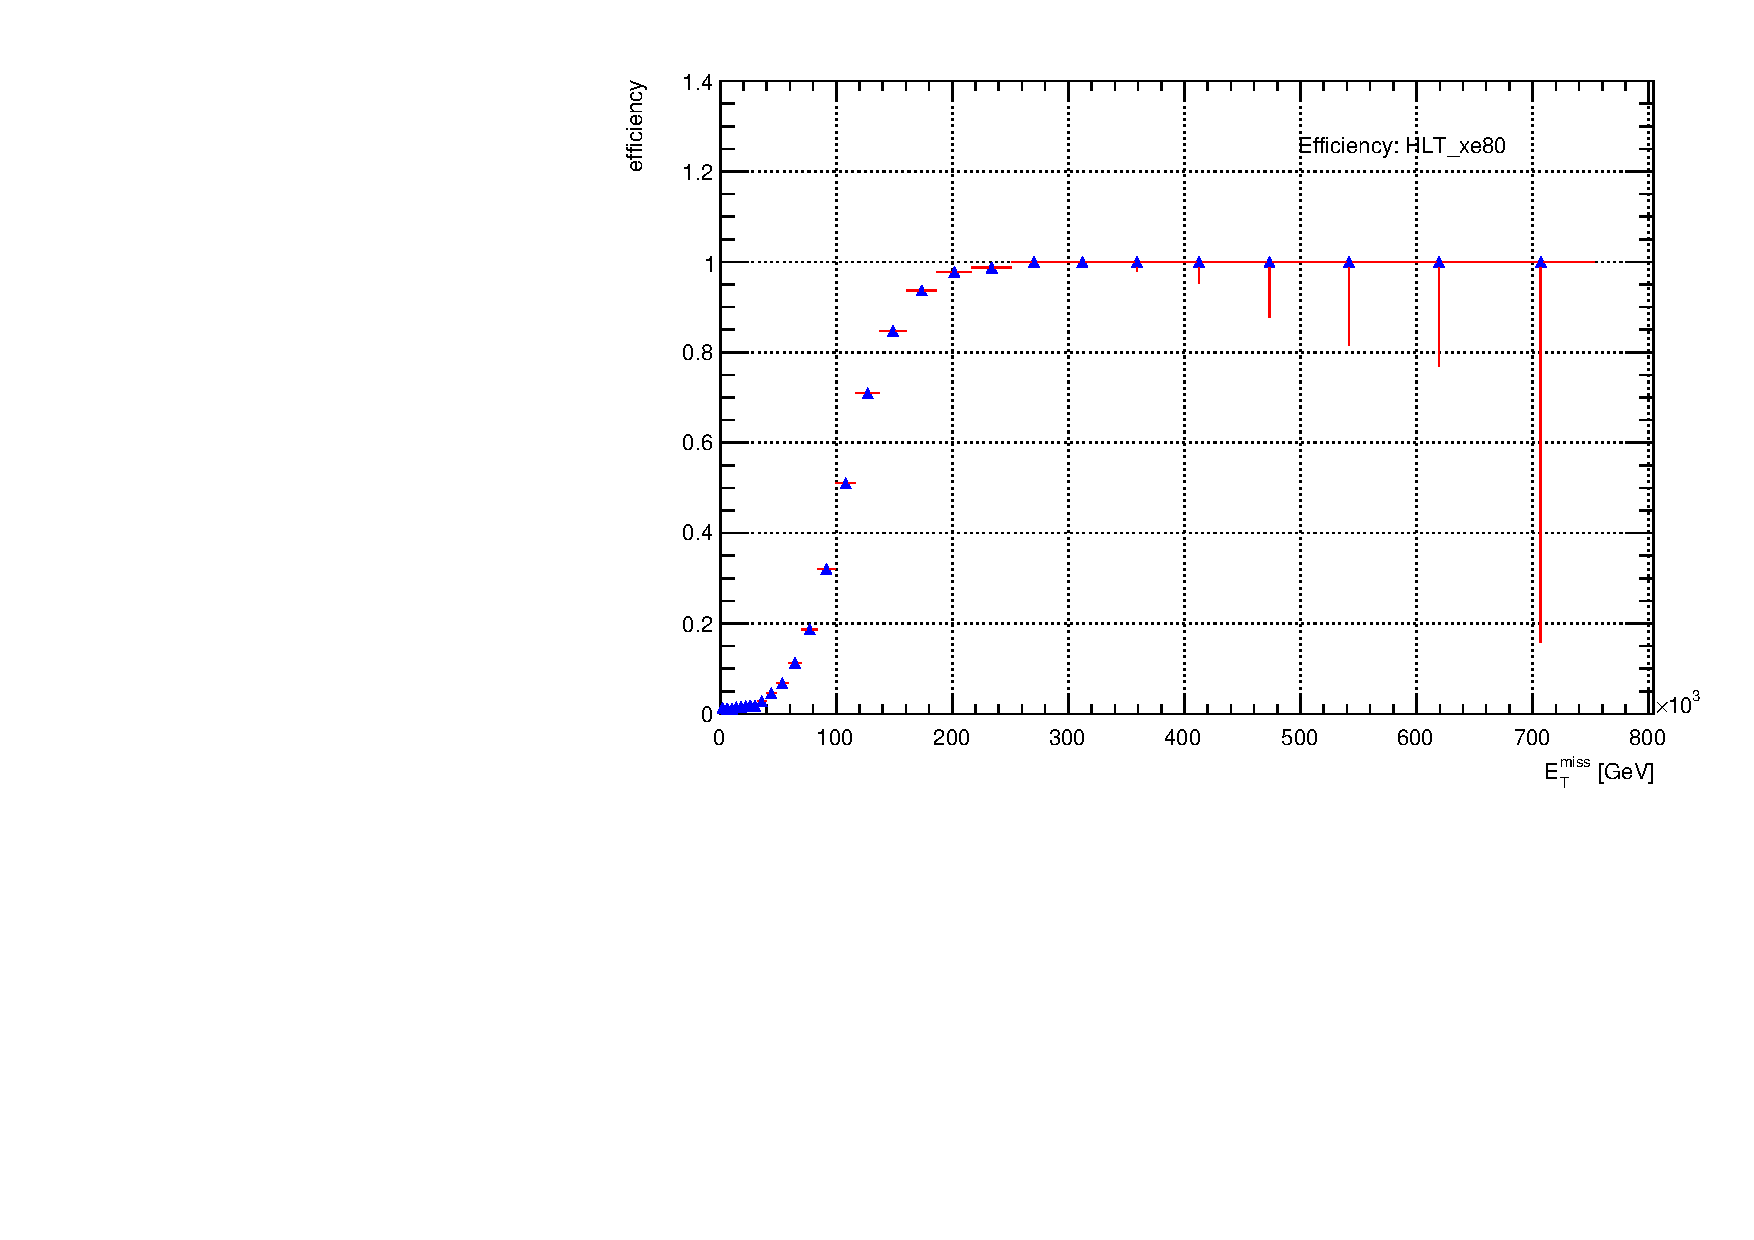
\includegraphics[width=0.42\textwidth]{TRIGGER/Eff_HLT_xe80_El_MC.pdf}}
\caption{Efficiency of \texttt{HLT\_xe80} versus the missing energy. All events were preselected for a muon-pair (left) or an electron-pair (right) ($\pt$> 10 GeV).}
\label{fig:eff_trigger3}
\end{figure}

\begin{figure}[h!]
\centering
\subfigure{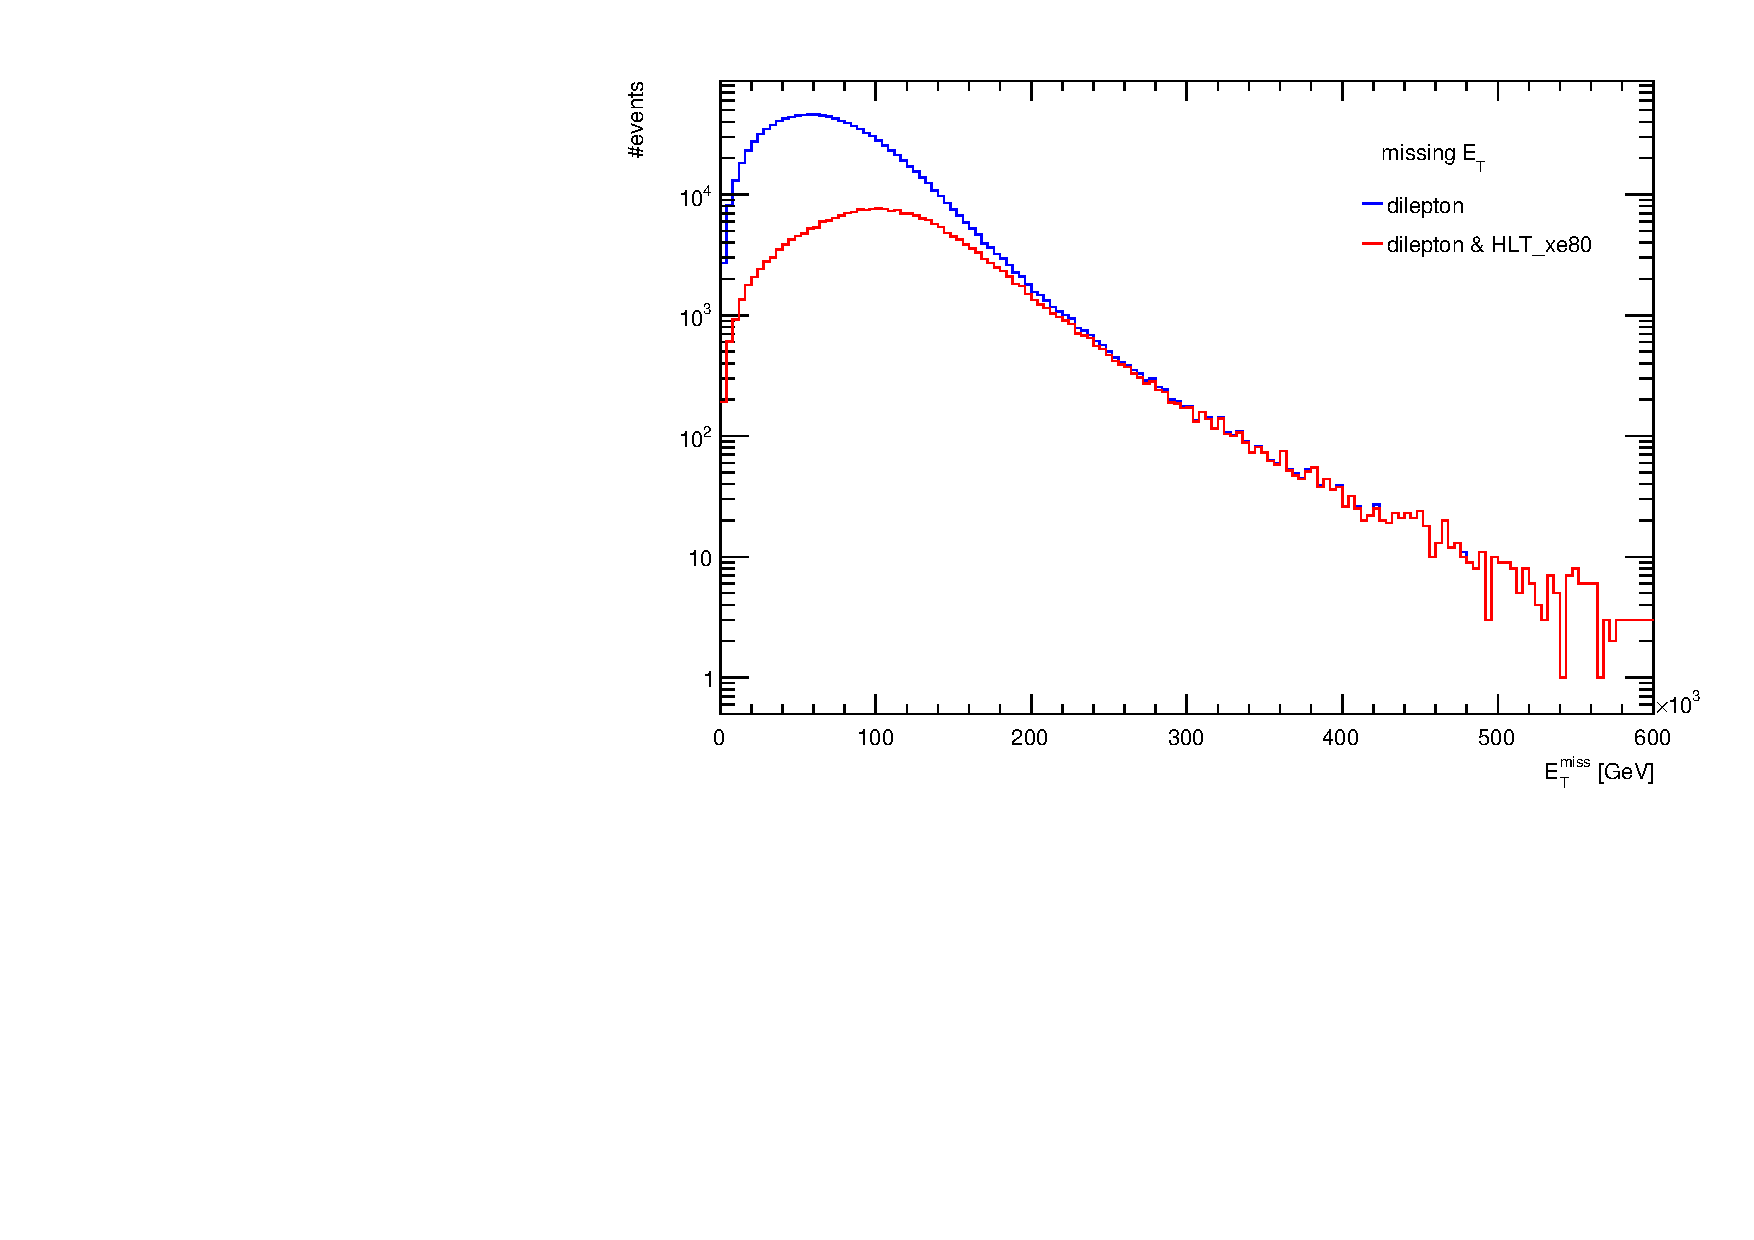
\includegraphics[width=0.42\textwidth]{TRIGGER/Events_HLT_xe80_MC.pdf}}
\subfigure{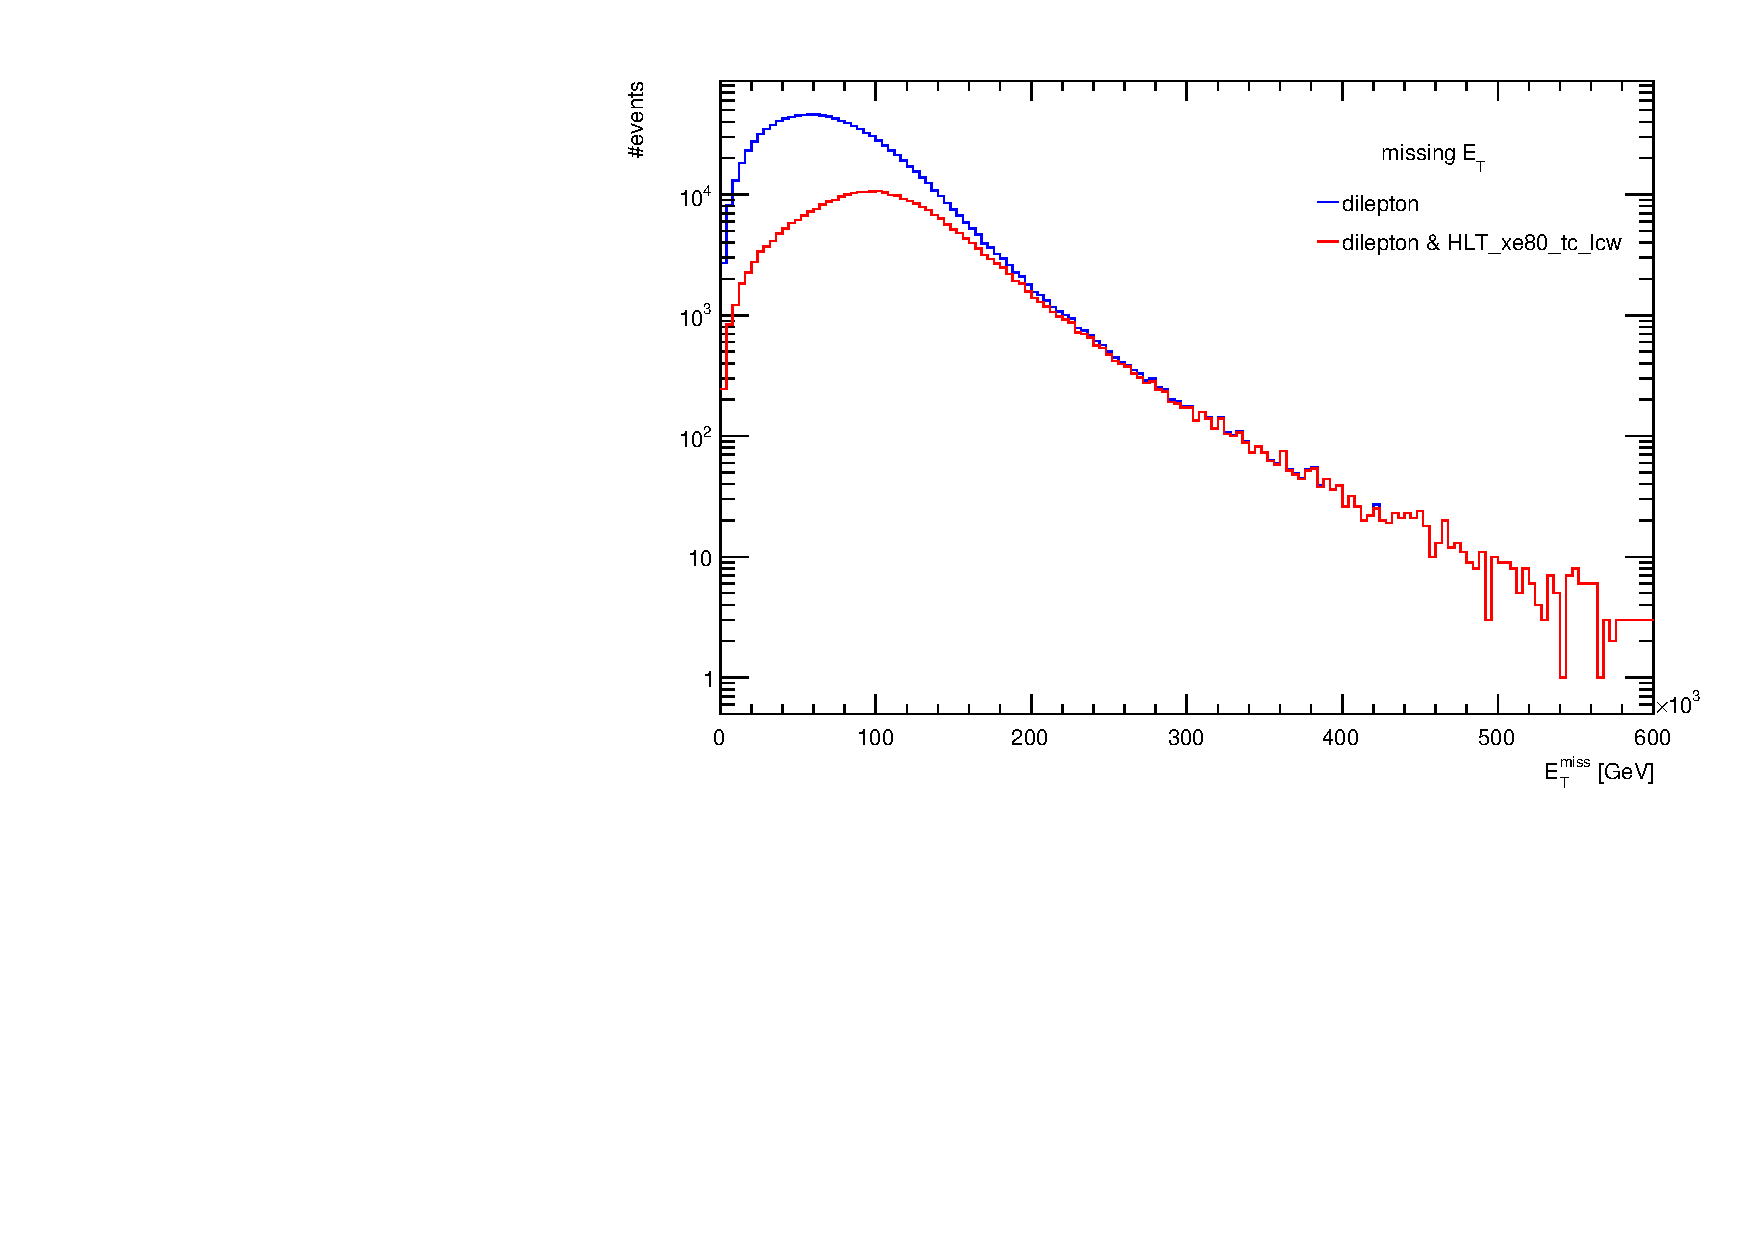
\includegraphics[width=0.42\textwidth]{TRIGGER/Events_HLT_xe80_tc_lcw_MC.pdf}}
\caption{Events selected by di-lepton triggers only and by an \texttt{AND} combination of di-lepton triggers and \texttt{HLT\_xe80} (left), \texttt{HLT\_xe80\_tc\_lcw} (right). Plotted against the missing energy.}
\label{fig:ev_trigger1}
\end{figure}

\begin{figure}[h!]
\centering
\subfigure{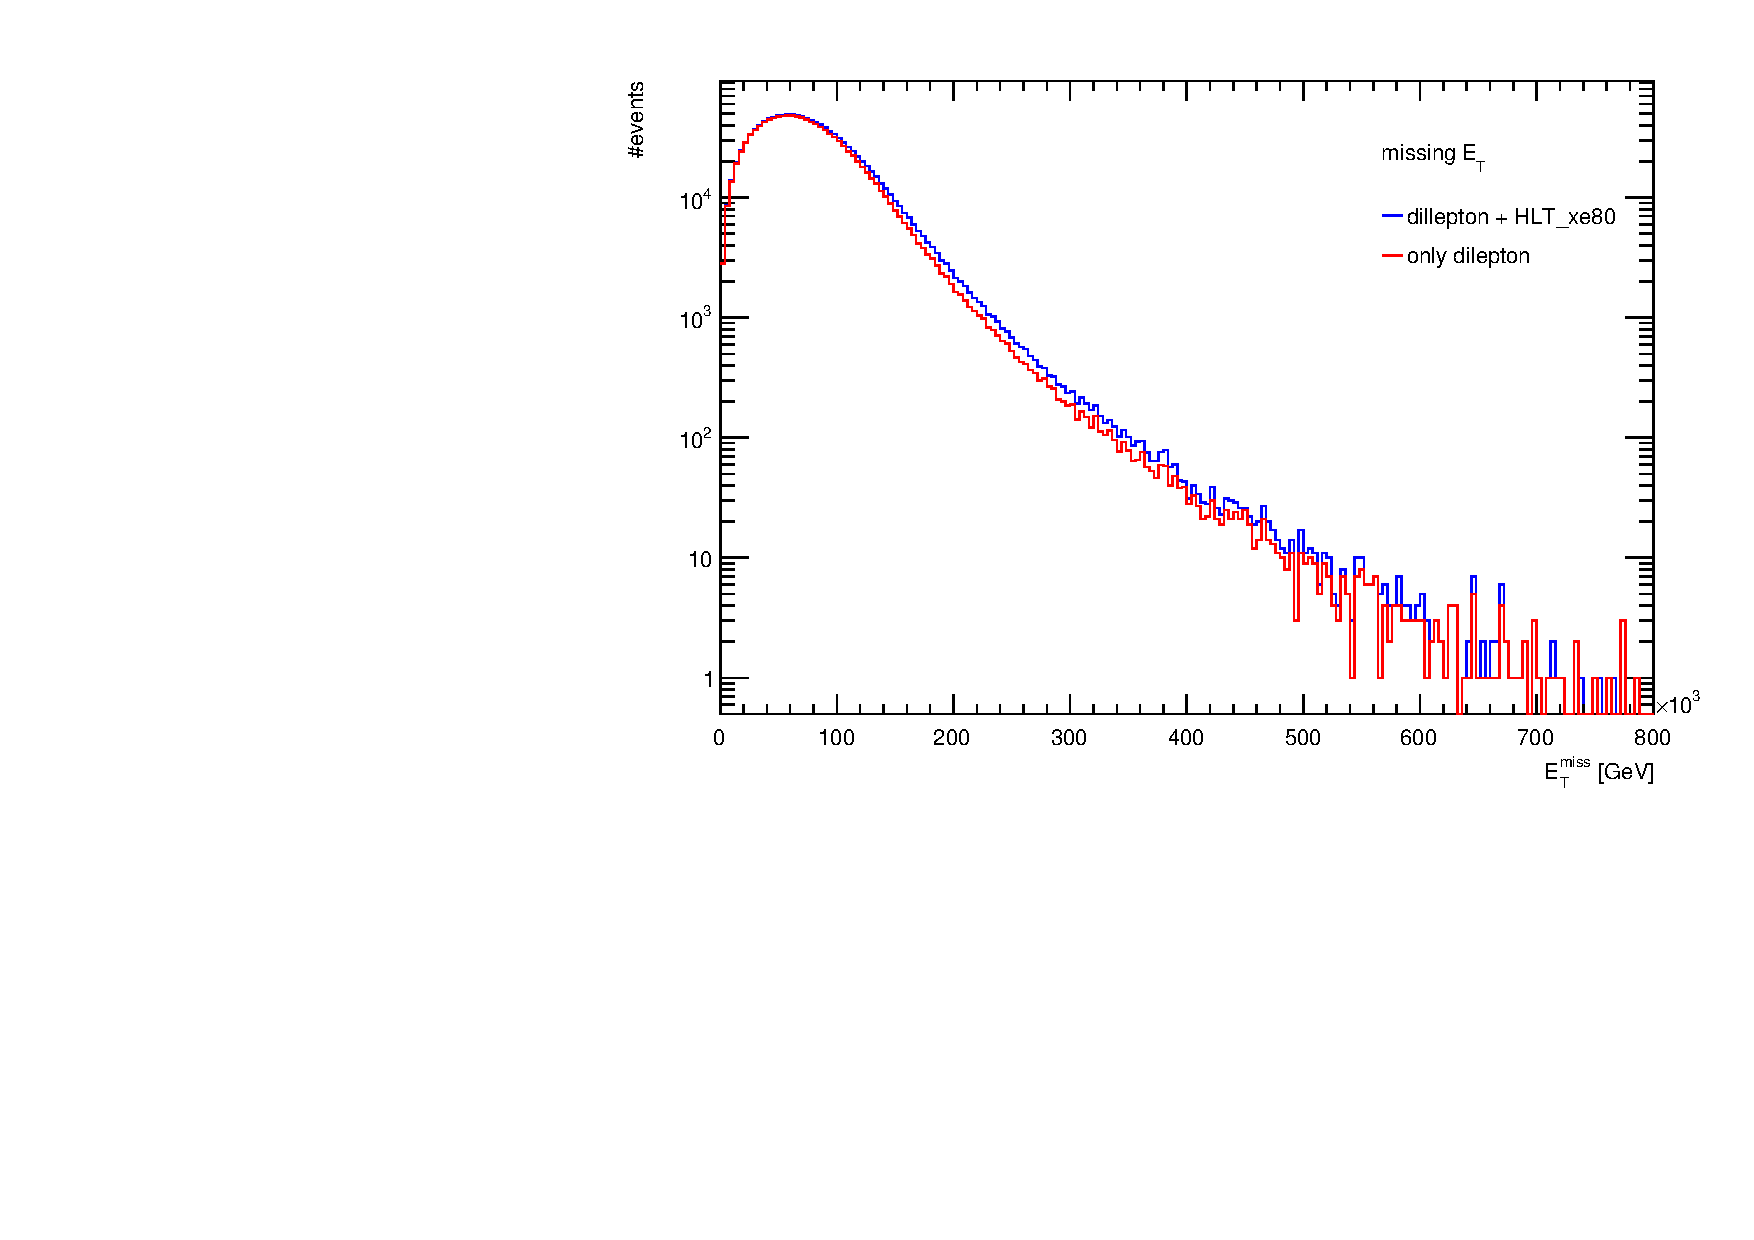
\includegraphics[width=0.43\textwidth]{TRIGGER/Events2_HLT_xe80_MC.pdf}}
\subfigure{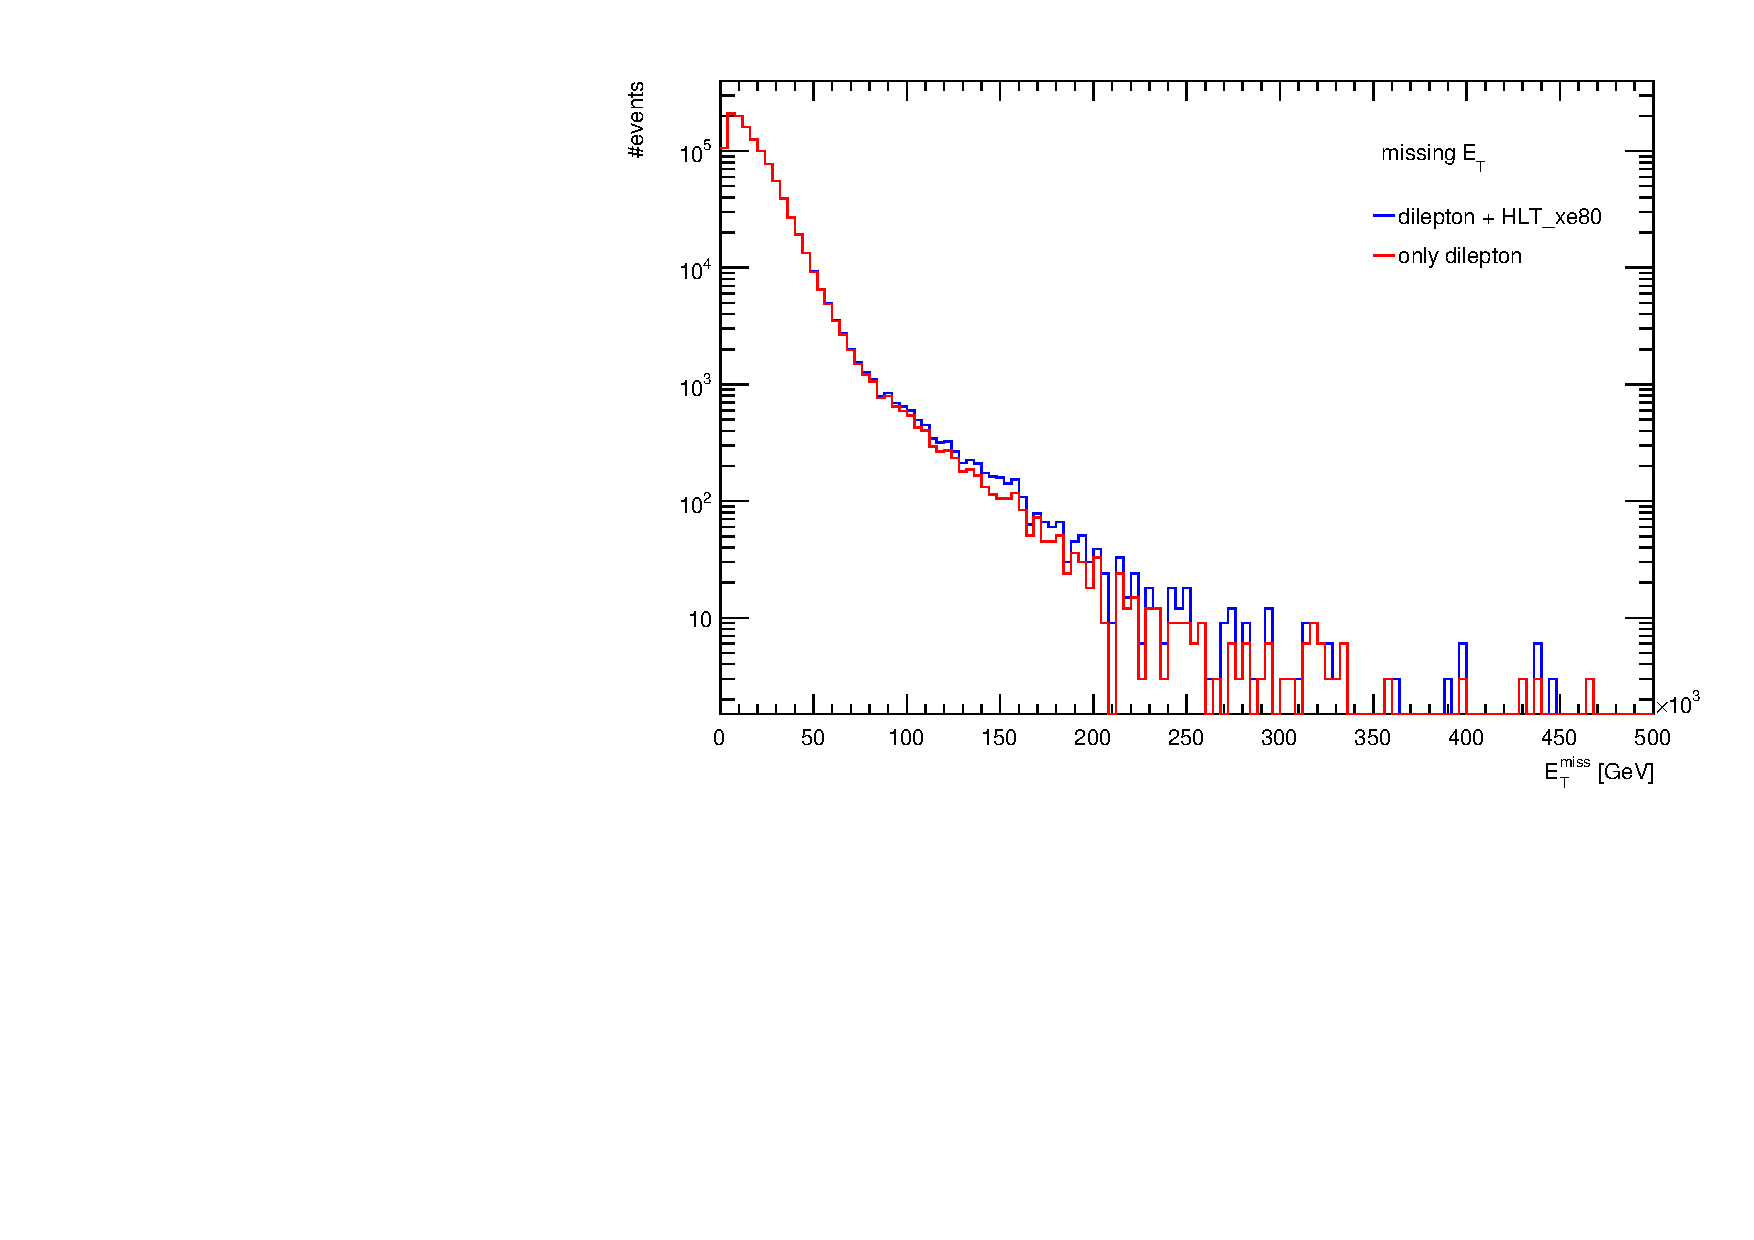
\includegraphics[width=0.43\textwidth]{TRIGGER/Events2_HLTxe80_Data.pdf}}
\caption{Events selected by di-lepton triggers only and by an \texttt{OR} combination of di-lepton triggers and \texttt{HLT\_xe80}. Shown for $t\bar{t}$ Monte Carlo (left) and for real data (right).}
\label{fig:ev_trigger2}
\end{figure}

\begin{figure}[h!]
\centering
\subfigure{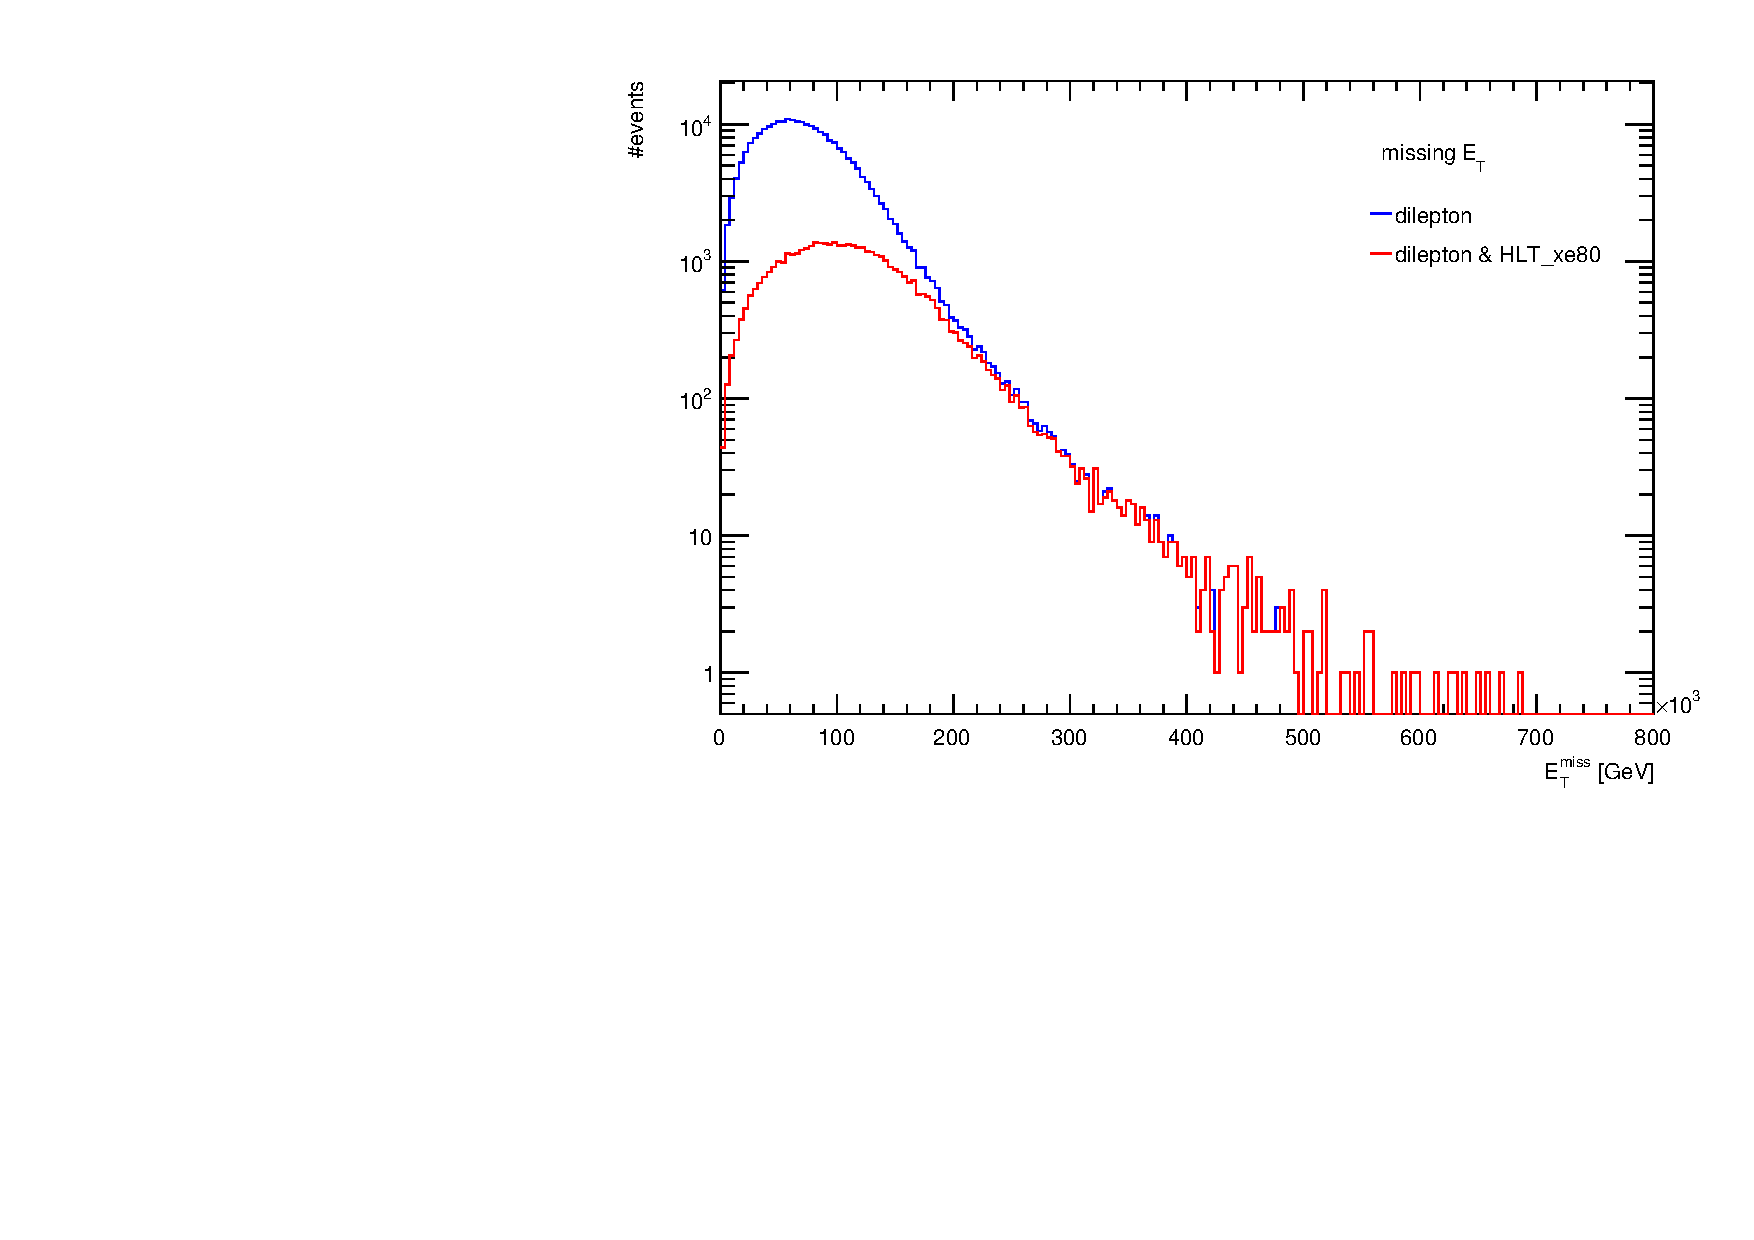
\includegraphics[width=0.43\textwidth]{TRIGGER/Events_HLT_xe80_Mu_MC.pdf}}
\subfigure{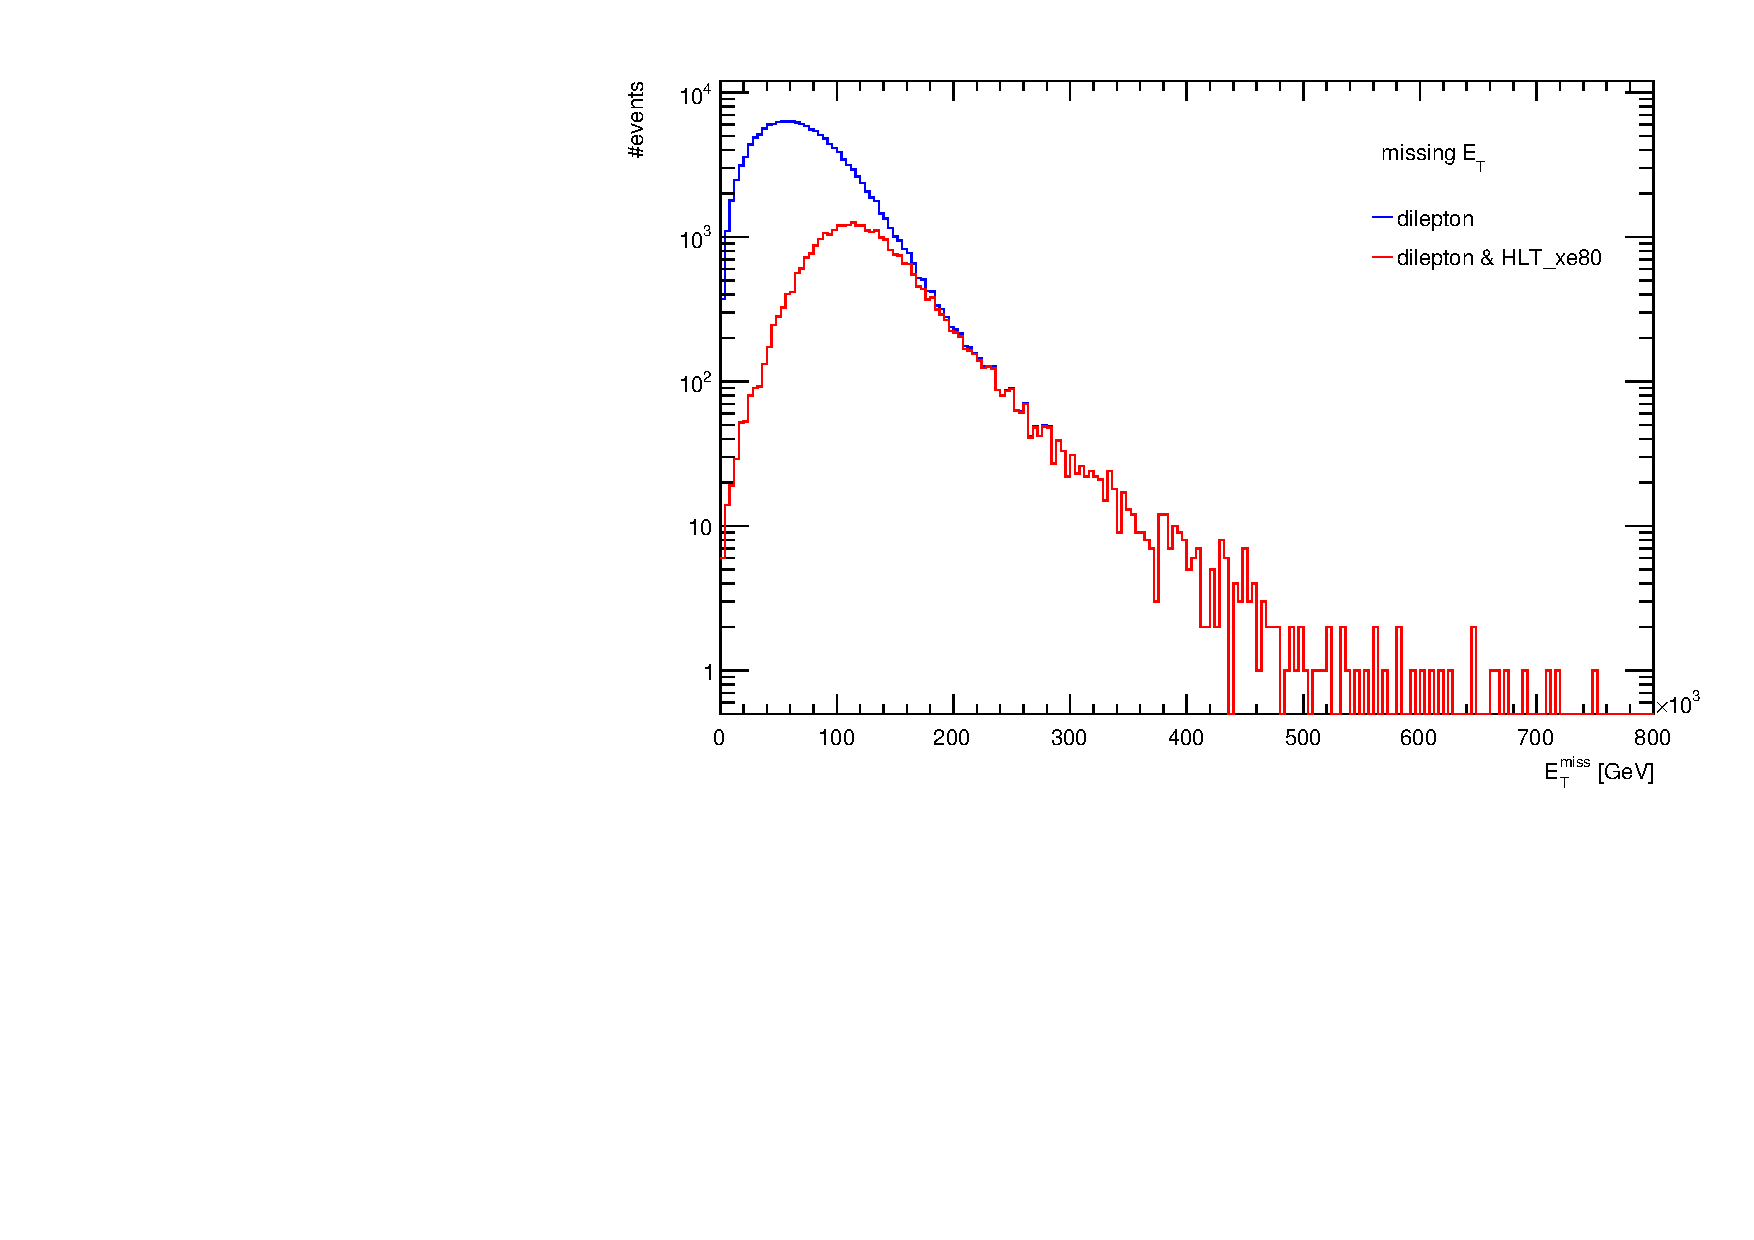
\includegraphics[width=0.43\textwidth]{TRIGGER/Events_HLT_xe80_El_MC.pdf}}
\caption{Events selected by di-lepton triggers only and by an \texttt{AND} combination of di-lepton triggers and \texttt{HLT\_xe80}. All events were preselected for a muon-pair (left) or an electron-pair (right) ($\pt$> 10 GeV). }
\label{fig:ev_trigger3}
\end{figure}


